%===============================================================================
% Zweck:    KTR-Seminar-Vorlage
% Erstellt: 16.10.2007
% Updated:  27.06.2016
% Autor:    U.K. / M.G.
%===============================================================================

%===============================================================================
% Zum Kompilieren pdflatex und bibtex ausführen.
% Konfiguration in texmaker: Options -> Configure Texmaker -> Quick Build -> Select Latexmk + ViewPDF
%	Entsprechende Informationen in den config/metainfo verändern
% Zur Auswahl der Sprache im folgenden Befehl
% ngerman für deutsch eintragen, english für Englisch.
%===============================================================================

\documentclass[journal, onecolumn, a4paper, 12pt]{IEEEtran}
%===============================================================================
% zentrale Layout-Angaben und Befehle
%===============================================================================
\newcommand\meta{../meta}
\input{\meta/config/commands}
%===============================================================================
% LATEX-Dokument
%===============================================================================

\input{\meta/config/hyphenation}

\usepackage{pdfpages}

\newcommand{\student}{Pio}
\makeatletter
\renewcommand\l@lstlisting[2]{\@dottedtocline{1}{1.5em}{2em}{#1}{#2}\vspace{1.2em}}
\makeatother
\begin{document}
%===============================================================================
% Zum Kompilieren pdflatex und bibtex ausführen.
% Konfiguration in texmaker: Options -> Configure Texmaker -> Quick Build -> Select Latexmk + ViewPDF
% Entsprechende Informationen in den config/metainfo verändern
% Zur Auswahl der Sprache im folgenden Befehl
% ngerman für deutsch eintragen, english für Englisch.
%===============================================================================
\selectlanguage{english}

\maketitle

\pagenumbering{Roman}
\setcounter{page}{2}
%
\tableofcontents
% Einstellungen f\"{u}r Literaturverzeichnis
\newpage
\addcontentsline{toc}{section}{\listfigurename}
\listoffigures
\newpage
\addcontentsline{toc}{section}{\listtablename}
\listoftables
\newpage
\addcontentsline{toc}{section}{\lstlistlistingname}
\lstlistoflistings
\newpage
\printnomenclature
%===============================================================================
% LATEX-Dokument: Kapitel laden
%===============================================================================
%
\newpage
\pagenumbering{arabic}
\setcounter{page}{1}

%
% to use git tagging
%
\ifgit
  \input{\meta/exampleContent/version}
\fi
%
% hier einzelne Kapitel mit \input{Kapitel-File} einf\"{u}gen
%
%\input{\meta/exampleContent/exampleContent}
\section{Introduction}
The rapid growth in the technology and information sector in recent years has resulted in a wide range of connectivity for various electronic and heterogeneous devices that can communicate effortlessly with each other over the Internet. Due to this technological improvement, termed as the Internet of Things (IoT), has made a gateway for various industrial sectors to inculcate IoT with varied applications that can rule over the Internet. \par

This technological improvement in recent years, especially in the Healthcare sector, has made video streaming in real-time improve our lives in tangible ways where one can monitor the other irrespective of the location. To achieve this goal, current multimedia streaming hardware devices are typically expensive. In order to provide improved and reliable services, we require low-cost hardware devices with easy deployment and high scalability that can be easily integrated into the already existing IoT networks. In our project, we use devices such as single-board computers (SBC) that enables video streaming using the Web Real-Time Communication (WebRTC) framework and peer-to-peer connection. \par

Our system built on Raspberry Pi (RPi) is completely packed into Docker Containers, which is easy to deploy using effective and readily available ARM architecture. It enables us to receive the video stream from the attached camera node and send it to the multimedia framework, which encodes, decodes, and sends it to the receiving device using a real-time communication protocol (RTP). We document the development of this system on RPi4 in this project paper.

\subsection{Goals} 
Our goal is to determine the best multimedia framework supported on the RPi by comparing the utilization of working video streams on RPi3 and RPi4 in terms of CPU usage, memory usage, and network throughput.

\subsection{Related Work}
Lukas and Vanessa’s \cite{lv} "WebRTC Surveillance Prototype on a Raspberry Pi" was the base for our project, where they were able to set up a video surveillance system based on peer-to-peer communication, which is deployed on a RPi3. This system support video streaming using the WebRTC framework and aiortc. They also compared different multimedia frameworks and codecs and concluded FFmpeg and GStreamer as the best using H.264 and Vp8 respectively. Based on this, we try to build the system on RPi4 and figure out the major difference in using RPi3 and RPi4 in terms of video streaming quality and resource utilization.
\section{Foundations for Our System}

%subsection1---------
\subsection{Hardware Technologies}

\subsubsection{Raspberry Pi}
The RPi\footnote{\url{https://en.wikipedia.org/wiki/Raspberry_Pi}} is a series of small SBCs which operates in an open-source ecosystem that features a Broadcom system on chip with integrated ARM architecture supported central processing unit (CPU) which is typically used in mobile phones and tablets. Due to its low-cost and availability, it provides high performance that puts the power of computing and digital making easier all over the world \cite{wiki}.\par

With various versions of RPi and evolved features, it is more widely used in many areas such as weather monitoring, learning programming skills, building hardware projects, home automation, and applications in various industries. It is a small and cheap computer that runs Linux but also provides a set of GPIO (general purpose input/output) pins that control the electronic components for physical computing and exploring the IoT \cite{Rpi}.

\subsubsection{Raspberry Pi 3 vs Raspberry Pi 4}
The RPi hardware has evolved through several versions that feature variations in the type of the CPU, memory capacity, networking support, and peripheral-device support \cite{wiki}. \par

Raspberry Pi 4: 
RPi version 4 has a lot of advantages from the previous models. The processing speed, multimedia performance, connectivity, memory speeds, and even the secure digital (SD) card read and write speeds are much faster, and the system as a whole is robust enough. It is available with three different memory sizes - 1GB, 2GB, and 4GB, support Dual 4k with USB 3.0 - to be the right fit for any project \cite{PI}. \par

Its main features are \cite{pi4vs3}: 
\begin{itemize}
	\item Processor: Broadcom BCM2711, Quad-core Cortex-A72 (ARM v8) 64-bit SoC @ 1.5GHz
	\item Memory: 1 GB, 2 GB, or 4 GB LPDDR4 SDRAM
	\item Connectivity: 802.11ac Wi-Fi, Gigabit Ethernet, Bluetooth 5.0
	\item Access: 40-pin GPIO header
	\item Video \& Sound: 2 x micro-HDMI, 3.5 mm analogue audio-video jack
	\item Multimedia: H.265 4Kp60, H.264 1080p60
	\item SD card support: microSD card
	\item Input power: 5V via USB type-C up to 3A and GPIO header up to 3A
\end{itemize}

Raspberry Pi 3:
Although RPi4 has extensible features, RPi3 is still on the go for its features like a full-size HDMI Port, More accessories (for now), and Gigabit Ethernet over USB 2.0. \par

Its main features are \cite{pi4vs3}:
\begin{itemize}
	\item Processor: Broadcom BCM2837B0 quad-core A53 (ARMv8) 64-bit @ 1.4GHz
	\item Memory: 1 GB LPDDR2 SDRAM
	\item Connectivity: 802.11ac Wi-Fi, 300Mbps Ethernet, Bluetooth 4.0
	\item Access: 40-pin GPIO header
	\item Video \& Sound: Full size – HDMI, 3.5 mm analogue audio-video jack
	\item Multimedia: H.264 \& MPEG-4 1080p30
	\item SD card: microSD card
	\item Input power: 5V via micro USB up to2.5A and GPIO header up to 3A
\end{itemize} 

%subsection2----------
\subsection{Software Technologies}

\subsubsection{WebRTC}
WebRTC is an open-source application that allows web browsers and mobile applications to communicate, transmit audio, video, and other generic data seamlessly through an Application Programming Interface (API) using a RTP. With WebRTC, most of the recent web browsers have built-in (Real-Time Communication) RTC functionality, which can find the best path for peer-2-peer connection, concealment of package loss, and echo cancellation during transmission, and built-in codecs for audio and video (U. Krieger: KTR-Mobicom-M-E, marcel Großmann), \cite{webrtc}. \par

There are three major APIs used in WebRTC (U. Krieger: KTR-Mobicom-M-E, marcel Großmann), \cite{webrtc}:
\begin{itemize}
	\item GetUserMedia: This enables the device to gain access to the camera, microphone, or screen of the device.
	\item peerConnection: This encodes and decodes the media and send it over the network, and takes care of the (Network Address Translation) NAT traversal.
	\item DataChannel: This creates the channel, sends  arbitrary data directly between the browsers with low latency. 
\end{itemize}

In sending of data between peers, the client browser M first sends a GET request to the web server, the web server confirms the request with Ok. Client browser L sends a GET request to the web server, which in succession it replies with Ok. The Client browser M negotiates with client browser L for media communication using a session description protocol (SDP). Once this negotiation is established, the web server creates a peer-to-peer connection between the two clients (U. Krieger: KTR-Mobicom-M-E, marcel Großmann), \cite{webrtc}. \par

In our project, WebRTC plays a very important role as the main goal is to stream video from a camera node over a WebRTC connection. The main advantage over the other (Internet Protocol) IP based video surveillance systems is that the network structure need not be configured manually nor the camera node or client require information before connecting, whereas in the case of IP based systems, they require cameras to be accessible via known public IP address or route video traffic through a server. Using WebRTC and peer-to-peer connection, traffic is sent between both peers directly if possible and routing is done dynamically. This allows for the flexible deployment of camera nodes with less or no configuration.

\subsubsection{Docker}
Docker is an OS-Level virtualization technology used to run a so-called container on the host. Containers are lightweight when compared to virtual machines that use lightweight kernel namespaces and runs on Build, Ship, and Run Paradigm. The main idea of containers is to collect all the tools and libraries necessary to run a specific piece of software, and then isolating that software from the rest of the system. Because containers are not full-on virtual machines, they are efficient, and Docker which is lightweight, standalone, is a leader in making containers easy to work \cite{8}. \par

In our project, we use Docker on RPi4 of 4GB RAM with a quad-core ARM processor of 1.5GHz to pack all the components into containers, which helps the system to be portable, modular and make deployment easy without any complicated steps. \par

We pull the image \textit{arm64v8/debian:buster-backports} from the registry to build the video streaming image. Then we run the video streaming containers.

%subsection3----------
\subsection{Multimedia Frameworks}
"A multimedia framework\footnote{\url{https://en.wikipedia.org/wiki/Multimedia_framework}} is a software framework that handles media on a computer and through a network \cite{mf}." Various multimedia frameworks are available, but we will only look at ones that are peculiar to our project.

\subsubsection{CVLC}
CVLC is an interfaceless VLC player \cite{cvlc}. It is an open-source multimedia framework, which is built-in with encoding, decoding, and transcoding libraries \cite{cvlc1}.

\subsubsection{FFmpeg}
FFmpeg\footnote{\url{http://ffmpeg.org/about.html}} is the term for Fast Forward MPEG, which can decode, encode, transcode, mux, demux, stream, filter, and play video streams.

\subsubsection{MJPG-Streamer}
MJPG-Streamer\footnote{\url{https://techvedika.com/mjpeg-linux-video-streaming-and-recording-over-http/}} is a command-line application. It copies JPEG frames from multiple inputs to multiple outputs. It streams a sequence of JPEG frames \cite{mjpgstreamer}. 

\subsubsection{GStreamer}
GStreamer\footnote{\url{https://en.wikipedia.org/wiki/GStreamer}} is an open-source multimedia framework that uses a pipeline-based workflow to combine different media processing systems. It reads files in one format, processes them, and exports them in another format \cite{gstreamer}. 

In our project, we use these four multimedia frameworks. For CVLC, and FFmpeg, we use two codecs H.264 and MJPEG, to encode the video stream. And for GStreamer we use H.264. The comparison of the multimedia frameworks and codecs is discussed in Sec. \ref{sec:4}

%subsection4----------
\subsection{Video Codecs}
"A video codec\footnote{\url{https://en.wikipedia.org/wiki/Video_codec}} is software or hardware that compresses and decompresses digital video \cite{videocodec}."

\subsubsection{H.264}
H.264\footnote{\url{https://www.streamingmedia.com/Articles/ReadArticle.aspx?ArticleID=74735}} is one of the standard video codecs which uses the DVD standard (MPEG-2) for the quality video image. It is also known for its maximum bitrate and resolution, which is good support for 4k and up to 8k Ultra High-Definition \cite{h264}.

\subsubsection{MJPEG}
MJPEG\footnote{\url{https://techvedika.com/mjpeg-linux-video-streaming-and-recording-over-http/}}, which is also known as Motion JPEG is a stream of JPEG images transferred over https protocol. The main advantage of MJPEG is that the installation of client software is not necessary on a remote host. The video stream can be seen in any software that supports MJPEG streaming (E.g., Google Chrome, Mozilla Firefox, VLC) \cite{mjpgstreamer}.

%subsection5----------
\newpage
\subsection{Tools}

\subsubsection{cAdvisor}
cAdvisor\footnote{\url{https://github.com/google/cadvisor}} also known as Container Advisor provides resource usage and performance traits of running containers. It collects, aggregates, processes, and exports information about running containers. It monitors complete resource usage and network statistics \cite{cadvisor}.

\subsubsection{Prometheus}
Prometheus\footnote{\url{https://en.wikipedia.org/wiki/Prometheus_(software)}} is an open-source software used for monitoring and alerting. It records metrics in real-time using predefined queries \cite{prometheus}. \par

\subsubsection{Jupyter Notebook}
"The Jupyter Notebook\footnote{\url{https://jupyter.org}} is an open-source web application that allows you to create and share documents that contain live code, equations, visualizations, and narrative text \cite{jn}."

%subsection6----------
\subsection{Versions of Hardware and Software Technologies}
The versions of hardware \& software technologies and tools we used in our project are listed below:
\begin{itemize}
   \item Raspberry Pi 3: Linux Black-pearl 4.19.58-hypriotos-v8, aarch64 1.2GHz ARM
   \item Raspberry Pi 4: Linux Black-pearl 4.19.102-v8, aarch64 1.5GHz ARM
   \item Docker: v18.09.7
   \item cAdvisor: v0.36.0
   \item Prometheus: v2.21.0
   \item Jupyter Notebook: v6.1.3
   \item Frameworks: arm64v8/debian:buster-backports v0.11
   \item Janus (WebRTC server): v0.10.3
\end{itemize}
\section{System Architecture and its Working}
\label{sec:three}

\subsection{Proposed Architecture for Video Streaming with Raspberry Pi's}

Our prototype for the project is based on the architecture consisting of RPi, camera node, client (receiving device), as shown in Fig. \ref{fig:archi}.

\begin{figure}[H]
	\centering
	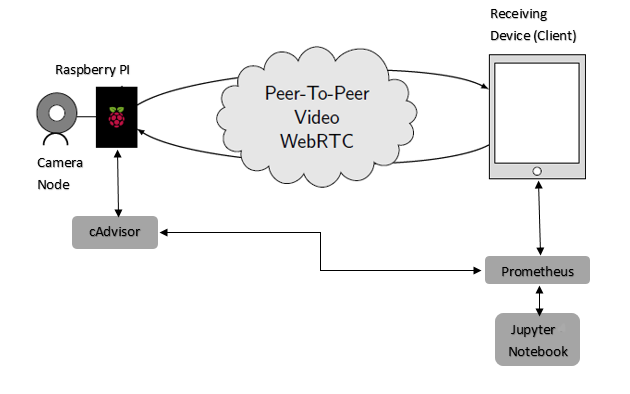
\includegraphics[width=\textwidth]{images/archi.png}
	\caption{System Architecture}
	\label{fig:archi}
\end{figure}


The main implementation in our project is built upon by running Docker containers to allow for easy deployment and management of its dependencies and starting all multimedia frameworks (CVLC, FFmpeg, MJPG-Streamer, GStreamer) with its codecs (H.264, MJPEG) on RPi. \par

We build all the necessary containers (frameworks and cAdvisor) on the RPi, where its respective Docker images are written in each of its Docker files. Navigate to each of the framework directories on RPi and start the framework by building and running Docker images, which it directs to its respective shell. We run the command to start the video streaming framework with specific encoders (H.264/MJPEG) in the shell. The workflow and commands for all the frameworks and codecs are explained in detail in Sec. \ref{sec:appendix}. \par

In order to view the video stream from RPi, a system (receiving device) that supports WebRTC peer-to-peer connection is integrated into the RPi network. Here we make use of VLC media player or web browser, based on the framework specification to view the video stream either through UDP (User Datagram Protocol) or TCP (Transmission Control Protocol) connection. \par

As our main goal in the project is to make a comparison between the multimedia frameworks and codecs in RPi3 and RPi4 based on the quality of video and resource utilization, we collect the statistics of the multimedia frameworks with its codecs from both RPi3 and RPi4 through cAdvisor (Container Advisor), a tool that exposes the raw data of resource usage and performance data of the running containers. \par

The workflow of cAdvisor in our project is as shown below: \par

To start cAdvisor, follow the steps shown in Code Listing. \ref{cadvisor}

\begin{lstlisting}[caption={Build and run cAdvisor}, frame=single, label={cadvisor}]
$docker run \
  --volume=/:/rootfs:ro \
  --volume=/var/run:/var/run:rw \
  --volume=/sys:/sys:ro \
  --volume=/var/lib/docker/:/var/lib/docker:ro \
  --volume=/dev/disk/:/dev/disk:ro \
  --publish=8080:8080 \
  --detach=true \
  --name=cadvisor \
  unibaktr/cadvisor
	
To view cAdvisor:
In browser: <Ip of the Rpi>:8080
\end{lstlisting}

\begin{figure}[H]
	\centering
	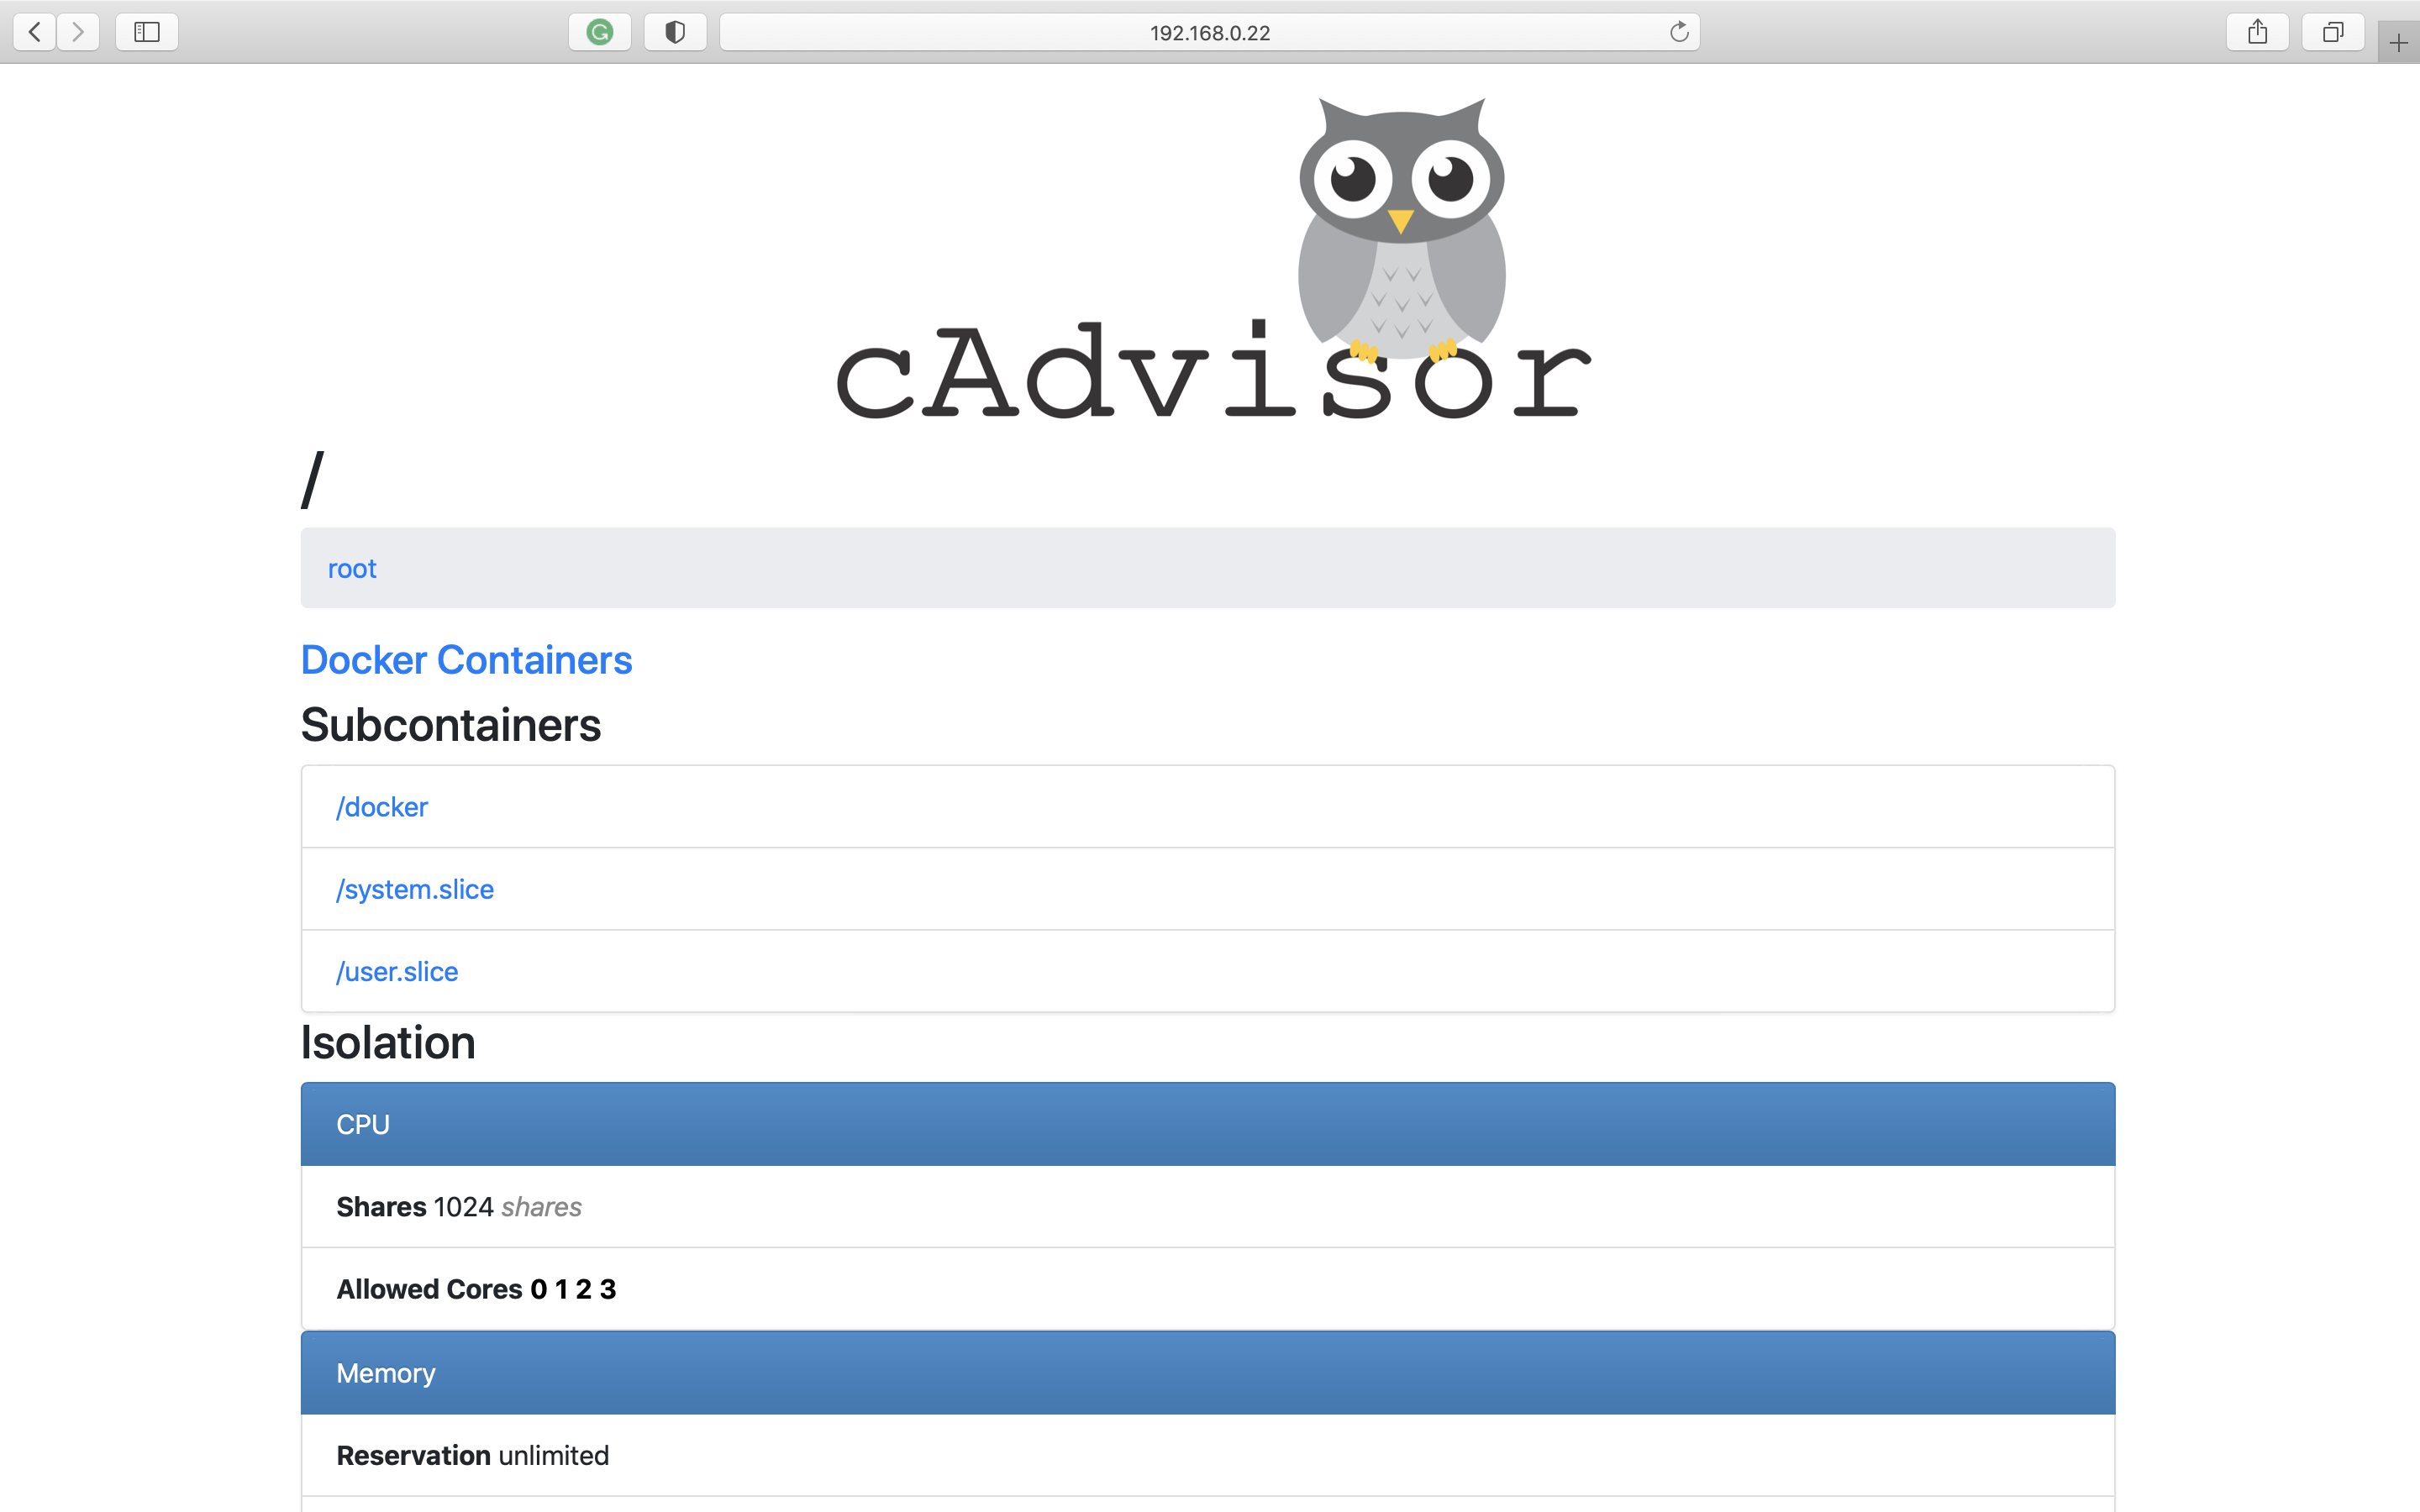
\includegraphics[width=\textwidth]{images/cAdvisor.png}
	\caption{cAdvisor}
	\label{fig:cAdvisor}
\end{figure}

Based on the statistics, to provide an easy, clear, and descriptive understanding of the data that has been generated, we make use of one of the graphical representations, \textbf{Boxplot}, to provide an illustration of values distributed based on mean, median, and maximum data more precisely in less space. \par

To draw the boxplot, we require the data to be present in a specific file format with its detailed statistics. As cAdvisor provides the raw data, we use \textbf{Prometheus}, an open-source software application used for monitoring and recording the metrics in real-time using pre-defined queries. In our case, Prometheus scrapes the exposed raw data metrics from cAdvisor using queries and saves the metrics to the file extension we require (in our case CSV file) locally. \par

The workflow of Prometheus in our project is as shown below: \par

You can run Prometheus on Docker, as the Prometheus services are available as Docker images.  

\begin{lstlisting}[caption={Dockerfile for Prometheus}, frame=single, label={prometheus1}]
FROM prom/prometheus
ADD prometheus.yml /etc/prometheus/
\end{lstlisting}

\begin{lstlisting}[caption={prometheus.yml file which consists of configuration}, frame=single, label={prometheus2}]
global:
  scrape_interval:15s
  scrape_timeout:10s
  evaluation_interval:20s
scrape_configs:
-job_name: cadvisor
  honor_timestamps:true
  scrape_interval:15s
  scrape_timeout:10s
  metrics_path: /metrics
  scheme: http
  static_configs:
  -targets:
    -<IP of the RPi>:8080
\end{lstlisting}

To build and run Prometheus on Docker, follow the steps shown in Code Listing. \ref{prometheus3}
\begin{lstlisting}[caption={Commands to build and run Prometheus on Docker}, frame=single, label={prometheus3}]
Navigate to the following directory:
/framework-test/ForReceiving_Device/Prometheus

$docker build -t my-prometheus .

$docker run -p 9090:9090 my-prometheus

To access the User Interface(UI) of the Prometheus:
In browser: <Ip of the Receiving Device>:9090
\end{lstlisting}

Once you build and run Prometheus, you can access the User Interface (UI) in the browser. Using predefined queries, you can narrow the metrics of a running container, as shown in Fig. \ref {fig:Prometheus UI}. Here, we are scraping the CPU usage of running container CVLC, which is using codec H.264 to stream the video.

\begin{figure}[H]
	\centering
	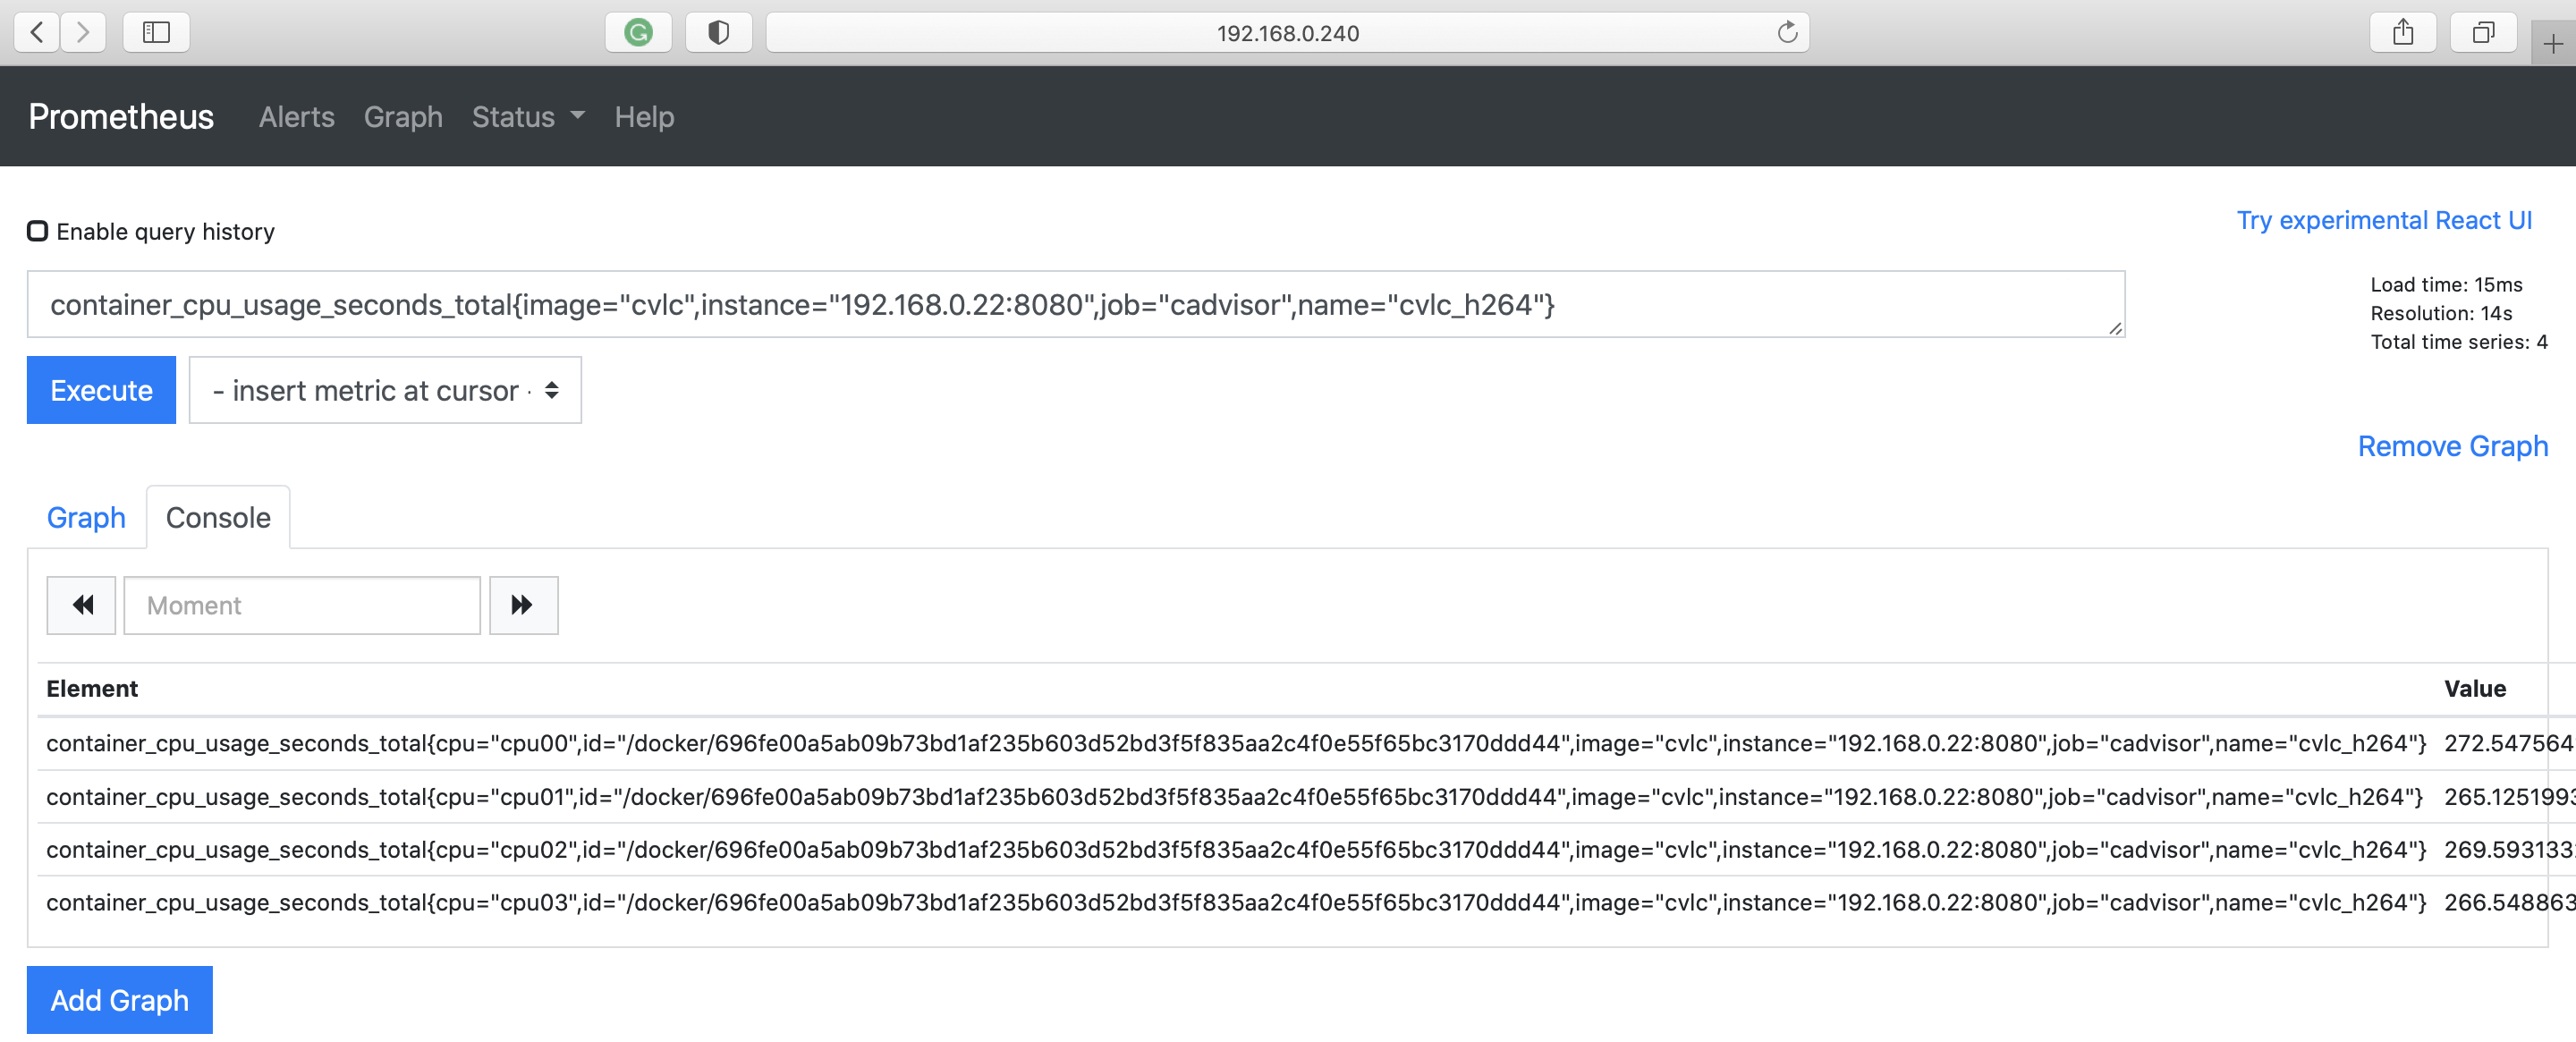
\includegraphics[width=\textwidth]{images/PrometheusUI.png}
	\caption{Prometheus UI}
	\label{fig:Prometheus UI}
\end{figure}

After narrowing down the metrics, we saved the metrics as a CSV file using Code Listing. \ref{prometheus4}. 

\begin{lstlisting}[style=mypython, caption={Python script to save the metrics as csv file}, frame=single, label={prometheus4}]
import csv
import requests
import sys

if len(sys.argv) != 3:
	print('Usage: {0} http://localhost:9090 a_query'.format(sys.argv[0]))
	sys.exit(1)

response = requests.get('{0}/api/v1/query'.format(sys.argv[1]), 
       params={'query':sys.argv[2]})
results = response.json()['data']['result']

# Build a list of all label names used
# gets all keys and discard _name_
labelnames = set()
for result in results:
	 labelnames.update(result['metric'].keys())

# Canonicalize
labelnames.discard('__name__')
labelnames = sorted(labelnames)

# Write the header
writer = csv.writer(sys.stdout)
writer.writerow(['name', 'timestamp', 'value'] + labelnames)

# Write the samples
for result in results:
	l = [result['metric'].get('__name__', '')] + result['value']
	for label in labelnames:
		l.append(result['metric'].get(label, ''))
		 writer.writerow(l)		
\end{lstlisting}

We run the Python script, as shown in Code Listing. \ref{prometheus5}. The Python file should be in the same directory where you are going to save the CSV files.

\begin{lstlisting}[caption={Run Python script}, frame=single, label={prometheus5}]
$python <name of python file>.py http://localhost:9090 
'container_cpu_usage_seconds_total{image="cvlc",instance="<IP of the RPi>",job=
"cadvisor",name="cvlc_h264"}' | gzip > $date +"%Y_%m_%d_%I_%M_%p")_gendata.gz
\end{lstlisting}

Once the data is scraped and saved locally to the file extension (CSV files), we use these files to plot the boxplot using \textbf{Jupyter Notebook}, an open-source web application that allows to create and share documents that contain live code, equation, visualizations, and narrative text. In our case, we use Jupyter Notebook to write Python scripts and draw the boxplot to give an illustration of comparison between RPi3 and RPi4 based on multimedia frameworks statistics. \par

The workflow of how we configure Jupyter Notebook and write Python scripts to draw the boxplot is shown below. \par

You can also run Jupyter Notebook on Docker, as the Jupyter Notebook services are also available as Docker images. 

\begin{lstlisting}[caption={Dockerfile for Jupyter Notebook}, frame=single, label={jp1}]
ARG BASE_CONTAINER=jupyter/datascience-notebook
FROM $BASE_CONTAINER
	
COPY . ./

WORKDIR $HOME
\end{lstlisting}

\begin{lstlisting}[caption={dockerBuild.sh}, frame=single, label={jp2}]
$docker build -t jupyter-notebook/hawk .
\end{lstlisting}

\begin{lstlisting}[caption={dockerRun.sh}, frame=single, label={jp3}]
$docker run \
 --env PORT=8888 \
 -it \
 -p 8888:8888 \
 jupyter-notebook/hawk
\end{lstlisting}

\begin{lstlisting}[caption={Build and run Jupyter Notebook on Docker}, frame=single, label={jp4}]
Navigate to the following directory:
/framework-test/ForReceiving_Device/jupyter-notebook
	
$./dockerBuild.sh
	
$./dockerRun.sh
\end{lstlisting}

Once you build and run Jupyter Notebook, you will get the URL to access the Jupyter Notebook server in the browser. Due to the ephemeral nature of Docker container, every saved notebook will be lost when we rebuild the container. So we dragged the necessary notebook files into the root directory of Jupyter, such that anytime we access the server, we could find the notebook which we already created.

\begin{figure}[H]
	\centering
	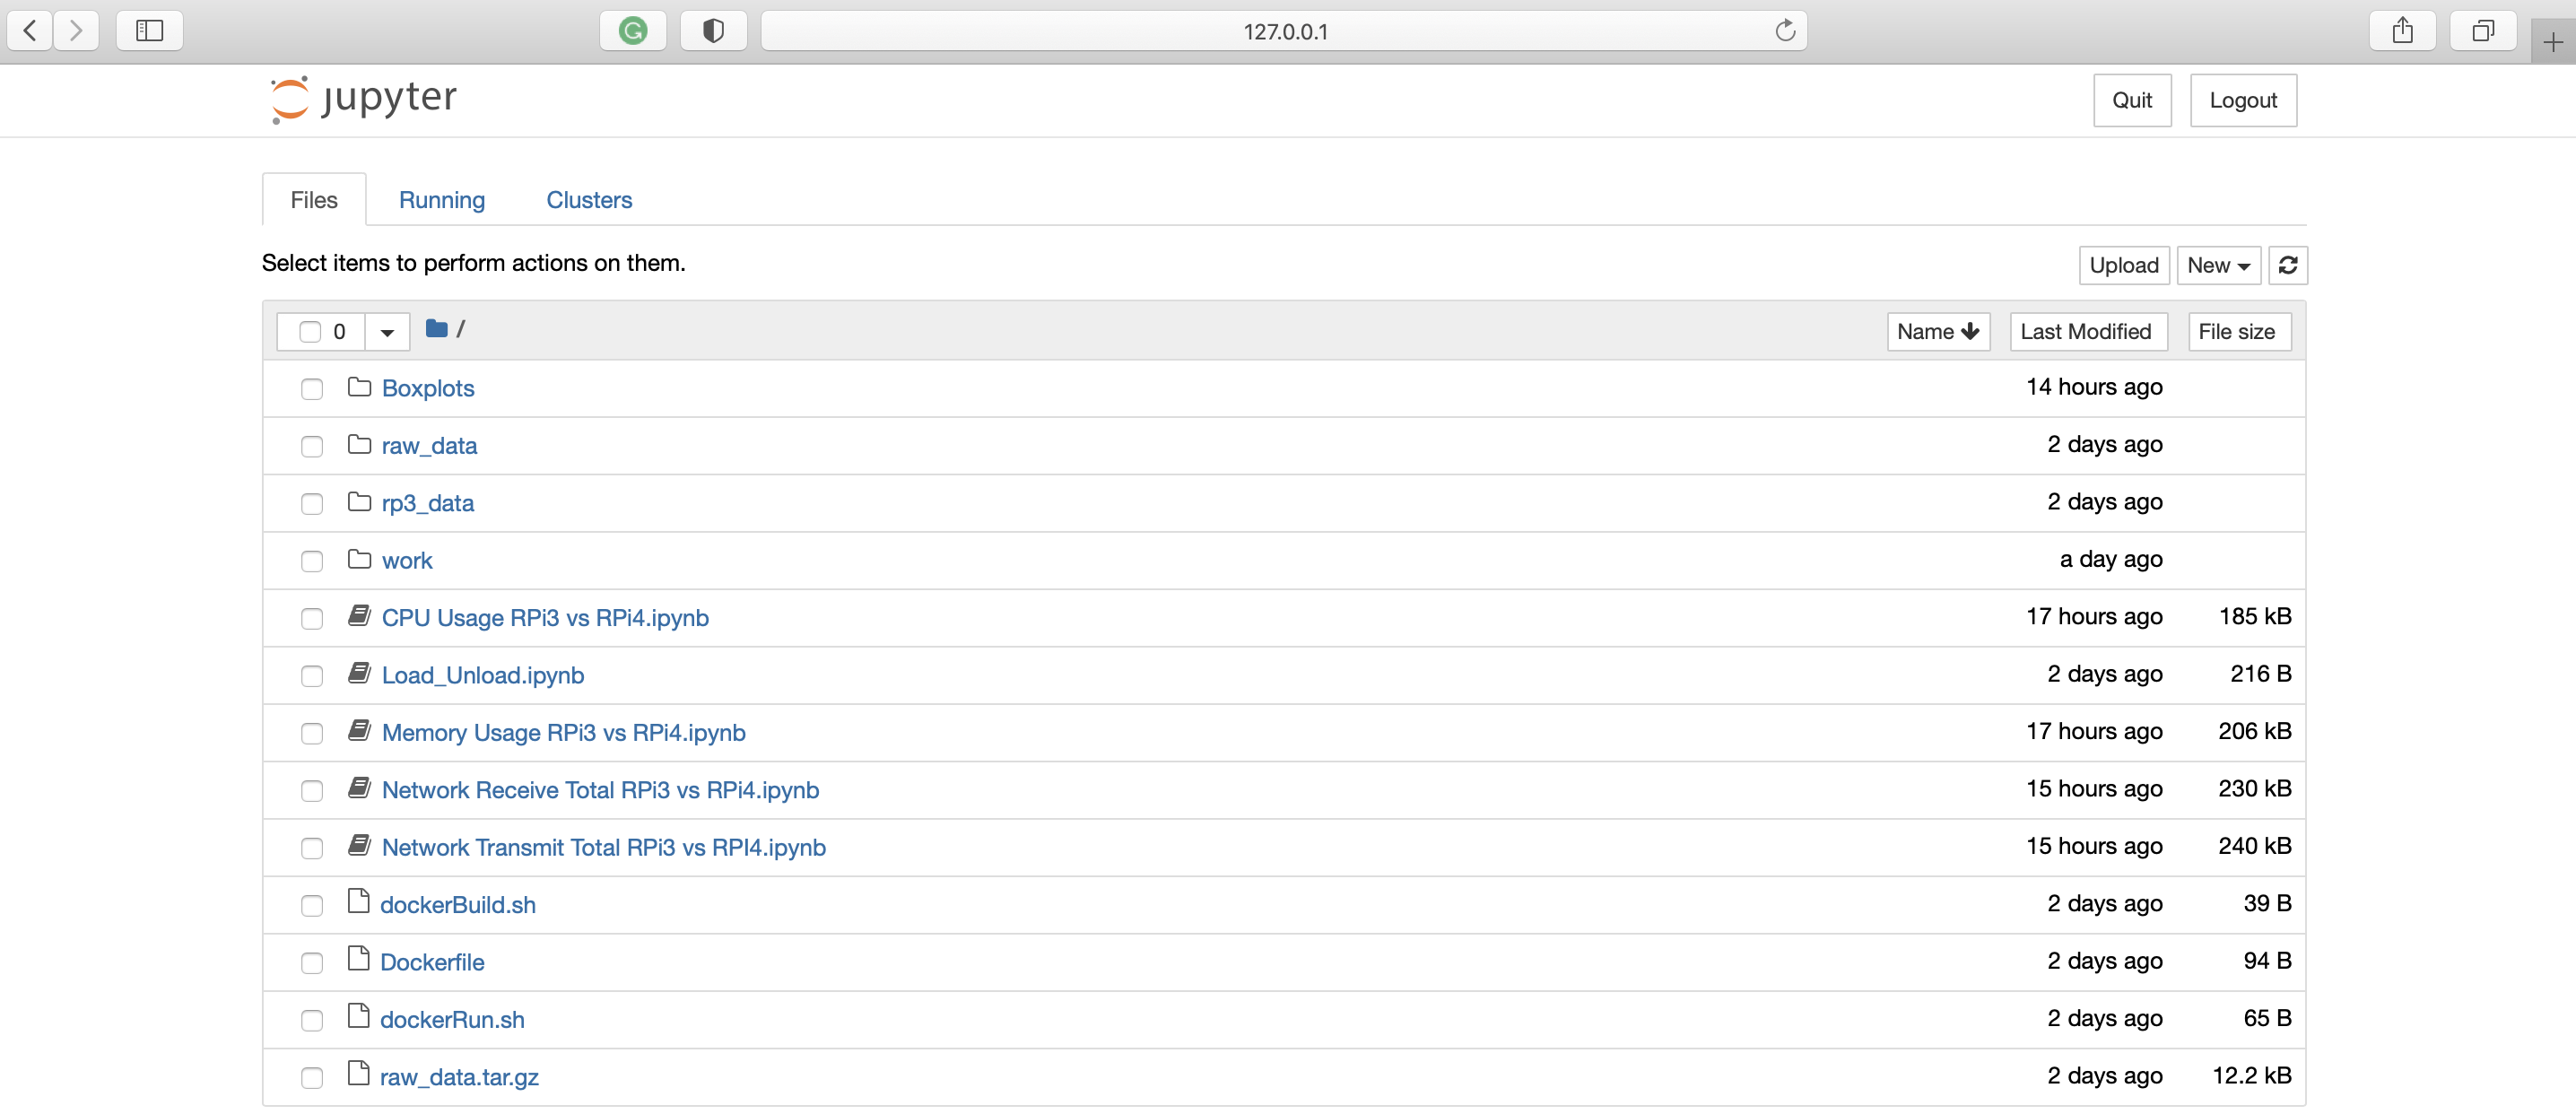
\includegraphics[width=\textwidth]{images/JupyterNotebookServer.png}
	\caption{Jupyter Notebook Server}
	\label{fig:Jupyter Notebook Server}
\end{figure}
\section{Evaluation of Multimedia Frameworks and Codecs}
\label{sec:4}

\subsection{Latency, Quality, and Resolution of Multimedia Frameworks and Codecs}

After evaluating the multimedia frameworks and its associated codecs, we arrive at the statistics of each of the video stream, and from these statistics, we analyze and come to a decision of which framework shows the best results. \par

As from the bitrate column in Table \ref{tab:table-stat}, MJPG-Streamer shows to be the best multimedia framework in our project. The number of processed bits within seconds determines the video quality. The higher the bitrate, the higher is the quality of the streaming video. In our case, MJPG-Streamer shows the best results followed by FFmpeg with the MJPEG codec.

\begin{table}[H]
	\begin{center}
	\caption{Statistics - Input}
	\label{tab:table-stat}
	\begin{tabular}{l | l | l | l | l}
		Frameworks and Codecs & Read at media & Input bitrate &  Demuxed & Stream bitrate \\
		\hline \hline
		cvlc h264 & 8211 KiB & 272 kb\slash s & 6221 KiB & 222 kb\slash s \\
		cvlc mjpeg & 108015 KiB & 3379 kb\slash s & 101973 KiB & 3268 kb\slash s \\
		ffmpeg h264 & 10300 KiB & 901 kb\slash s & 9313 kb\slash s & 830 kb\slash s \\
		ffmpeg mjpeg & 16544 KiB & 1283 kb\slash s & 16495 KiB & 1345 kb\slash s \\
		mjpgstreamer & 80031 KiB & 7301 kb\slash s & 79814 KiB & 7575 kb\slash s   
	\end{tabular}
	\end{center}
\end{table}

The video streams are formed by a sequence of frames which are calculated per given time unit. The higher the frame rate, the smoother the video will be. Table \ref{tab:videoframe} shows the video frame rate, each video streaming framework displays per given time, and the number of lost frames. From the statistics, we can say that there is a higher number of lost frames in CVLC, which can be due to network and bitrate fluctuation.

\begin{table}[H]
	\begin{center}
		\caption{Statistics - Video}
		\label{tab:videoframe}
	\begin{tabular}{l | l | l | l}
		Frameworks and Codecs & Decoded blocks & Displayed frames & Lost frames \\
		\hline \hline
		cvlc h264 & 16.487 & 8.243 & 27 \\
		cvlc mjpeg & 32.765 & 18.002 & 97 \\
		ffmpeg h264 & 4.177 & 2.067 & 0 \\
		ffmpeg mjpeg & 4.710 & 2.376 & 0 \\
		mjpgstreamer & 4.314 & 2.162 & 0 
	\end{tabular}
\end{center}
\end{table} 

Among the two video codecs (H.264, MJPEG) we used, H.264 compresses chunks of video frames at once, whereas MJPEG compresses video frames as a sequence of JPEG images. From Table \ref{tab:videocodec}, we can say that H.264 compresses chunks of video frames, whereas MJPEG has no frame rate as it compresses video frames sequentially. Coming to the video resolution MJPG-Streamer shows High-Definition (HD) video because of its high resolution.

\begin{table}[H]
	\begin{center}
		\caption{Codec details}
		\label{tab:videocodec}
	\begin{tabular}{l | l | l }
		Frameworks and Codecs & Video resolution & Frame rate \\
		\hline \hline
		cvlc h264 & 640x354 & 24\\
		cvlc mjpeg & 752x416 & \\
		ffmpeg h264 & 752x416 & 25\\
		ffmpeg mjpeg & 752x416 & \\
		mjpgstreamer & 1280x720 & 
	\end{tabular}
\end{center}
\end{table}

GStreamer can interconnect with other multimedia frameworks using their available libraries such as codecs. In our project, VLC does not support GStreamer and can only view the video stream on the web browser when it is streamed through a Janus (WebRTC server). Janus, on the other hand, supports multimedia frameworks, such as GStreamer, FFmpeg, etc, and video codecs H.264 and Vp8.

\subsubsection{Video Quality and Resolution of Working Video Streams}

The quality was evaluated with subject to each of the frameworks (see Fig. \ref{fig:cvlc1}, \ref{fig:cvlc2}, \ref{fig:ffmpeg1}, \ref{fig:ffmpeg2}, \ref{fig:mjpg}), and latency was measured by making single short movements in front of the camera and finding the difference between real movements and its appearance in the stream. The pictures of the resolution and the quality of the video streams are shown below: \par

%Fig. \ref{fig:ffmpeg2} shows poor quality in the video due to the high latency and loss of frames during transmission even though the network throughput was equal to the sent video frame rate.

\begin{figure}[ht]
\centering \begin{minipage}[b]{0.45\linewidth}
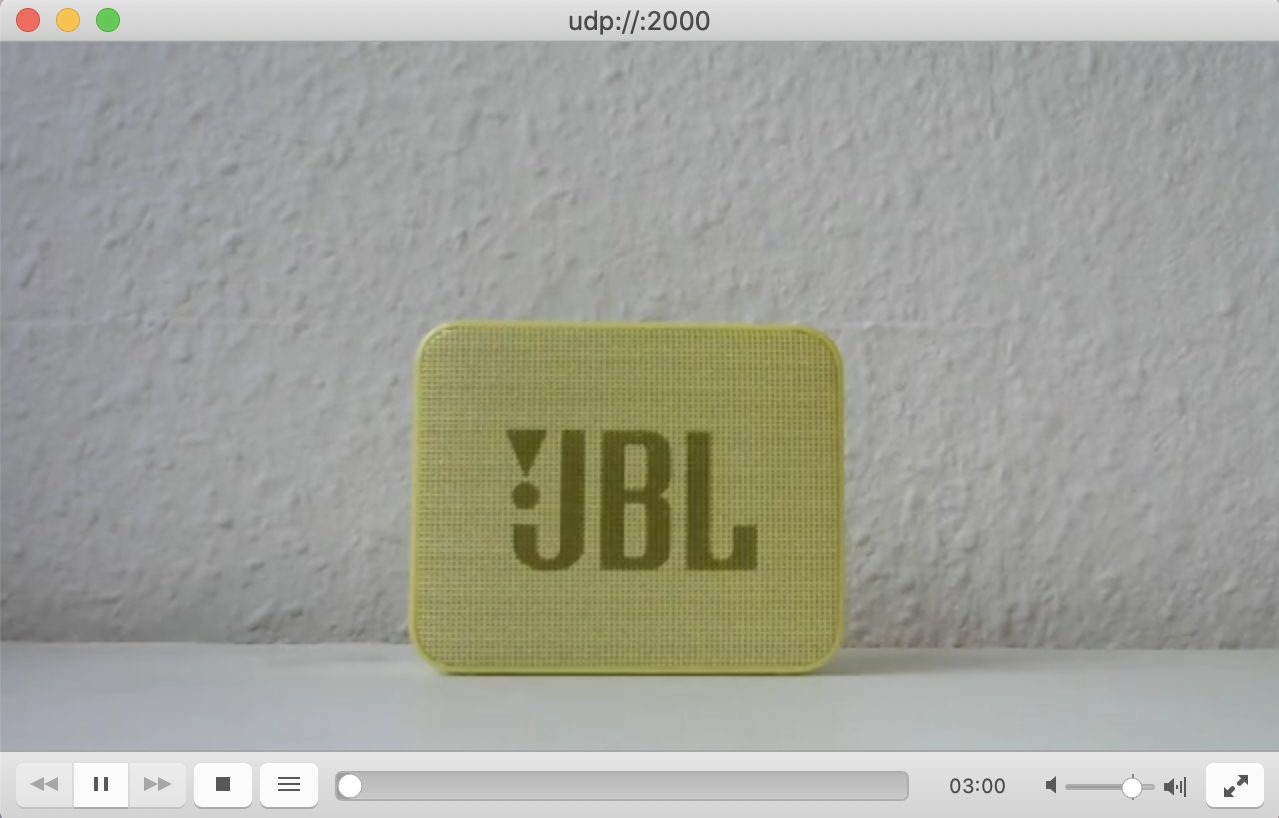
\includegraphics[width=\textwidth]{images/CVLC_H.264.png}
\caption{CVLC H.264} \label{fig:cvlc1}
\end{minipage}
\quad \begin{minipage}[b]{0.45\linewidth}
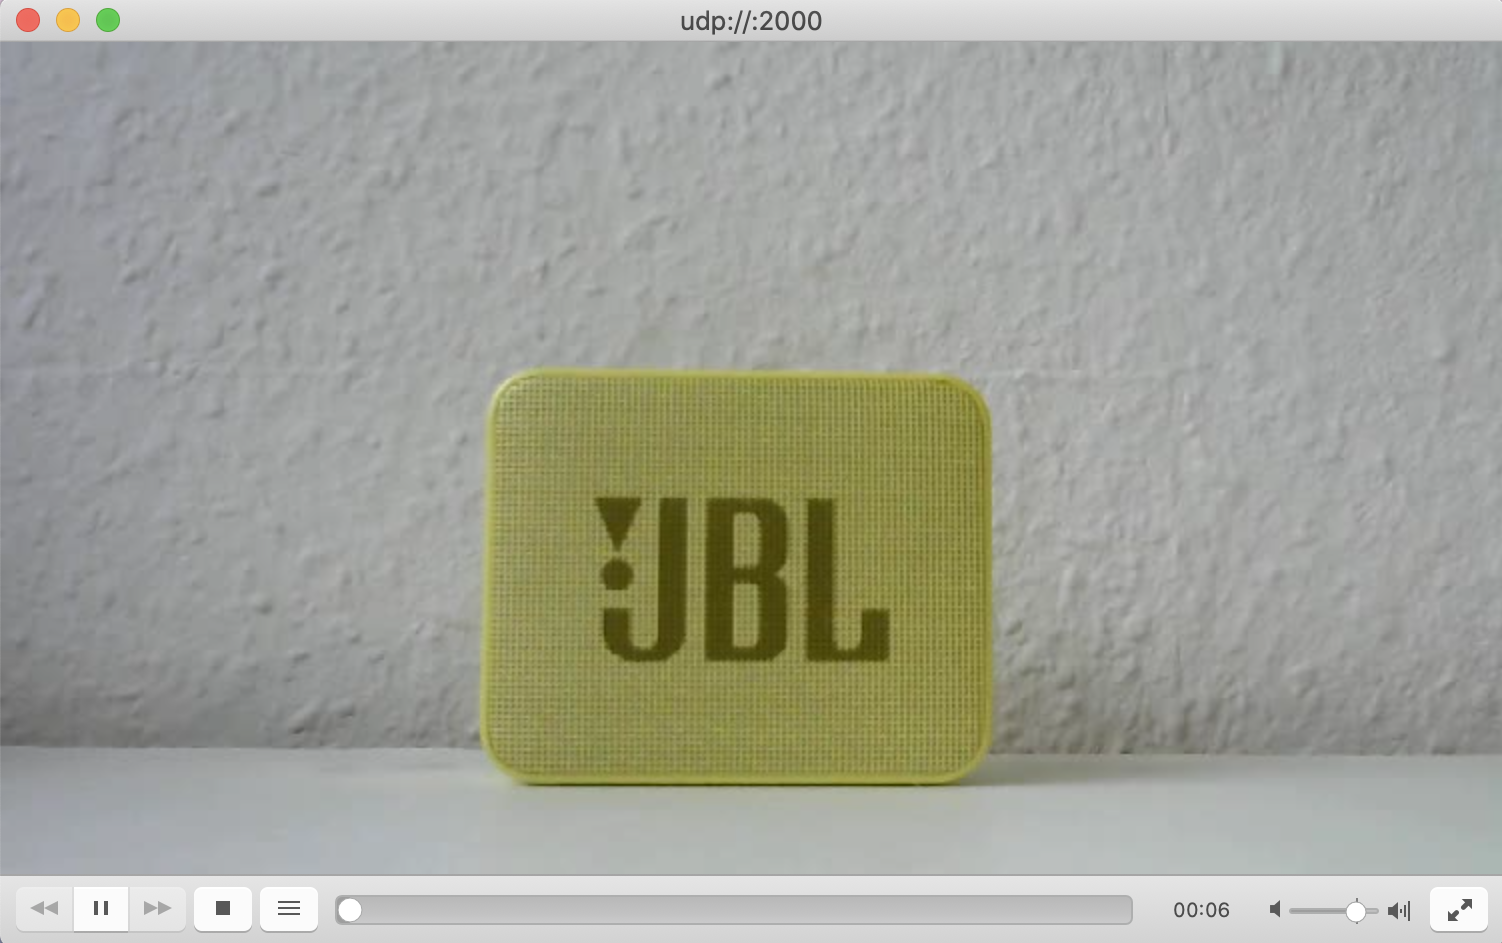
\includegraphics[width=\textwidth]{images/CVLC_MJPEG.png}
\caption{CVLC MJPEG} \label{fig:cvlc2}
\end{minipage}
\end{figure}

\begin{figure}[ht]
\centering \begin{minipage}[b]{0.45\linewidth}
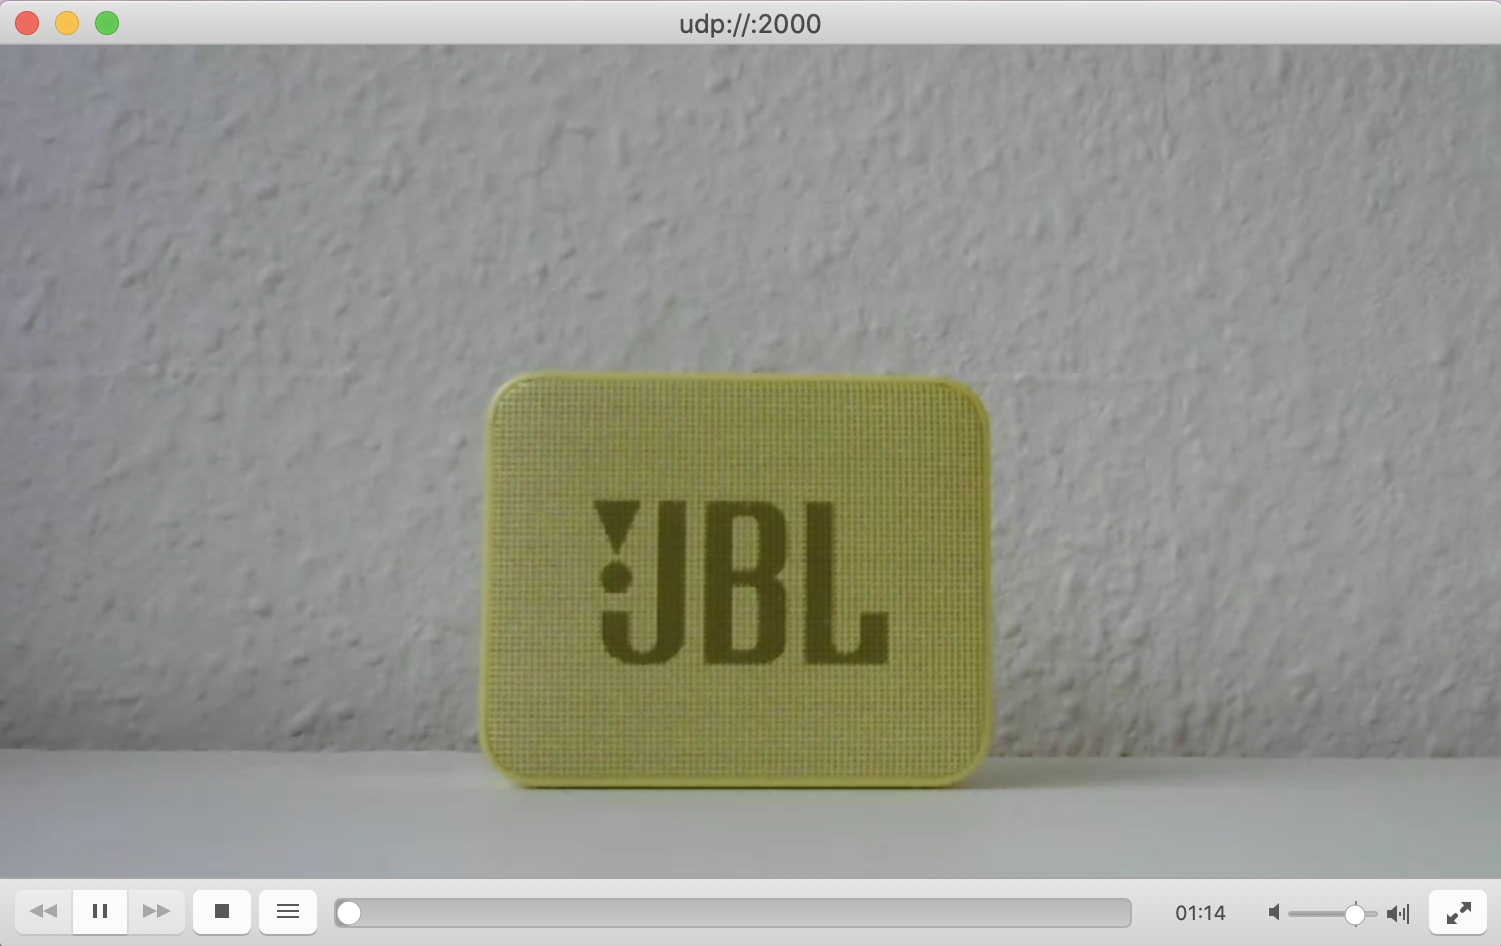
\includegraphics[width=\textwidth]{images/FFmpeg_H.264.png}
\caption{FFmpeg H.264} \label{fig:ffmpeg1}
\end{minipage}
\quad \begin{minipage}[b]{0.45\linewidth}
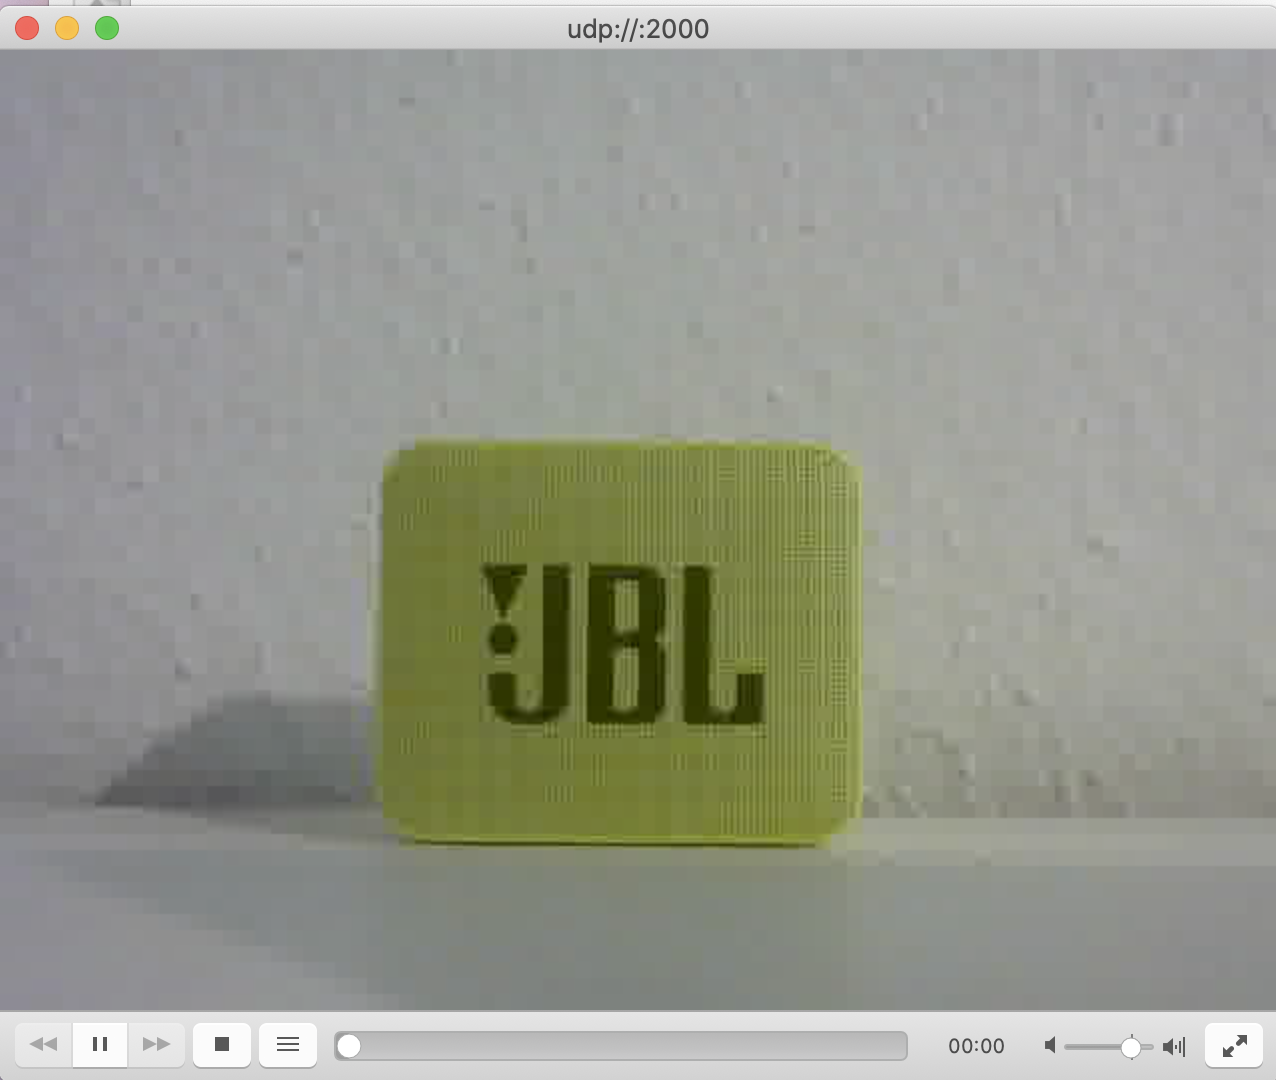
\includegraphics[width=\textwidth]{images/FFmpeg_MJPEG.png}
\caption{FFmpeg MJPEG} \label{fig:ffmpeg2}
\end{minipage}
\end{figure}

\newpage
Fig. \ref{fig:mjpg} of MJPG-Streamer shows a better video quality among all the frameworks because of its high resolution followed by is the FFmpeg with MJPEG (Fig. \ref{fig:ffmpeg2})

\begin{figure}[H]
	\centering
	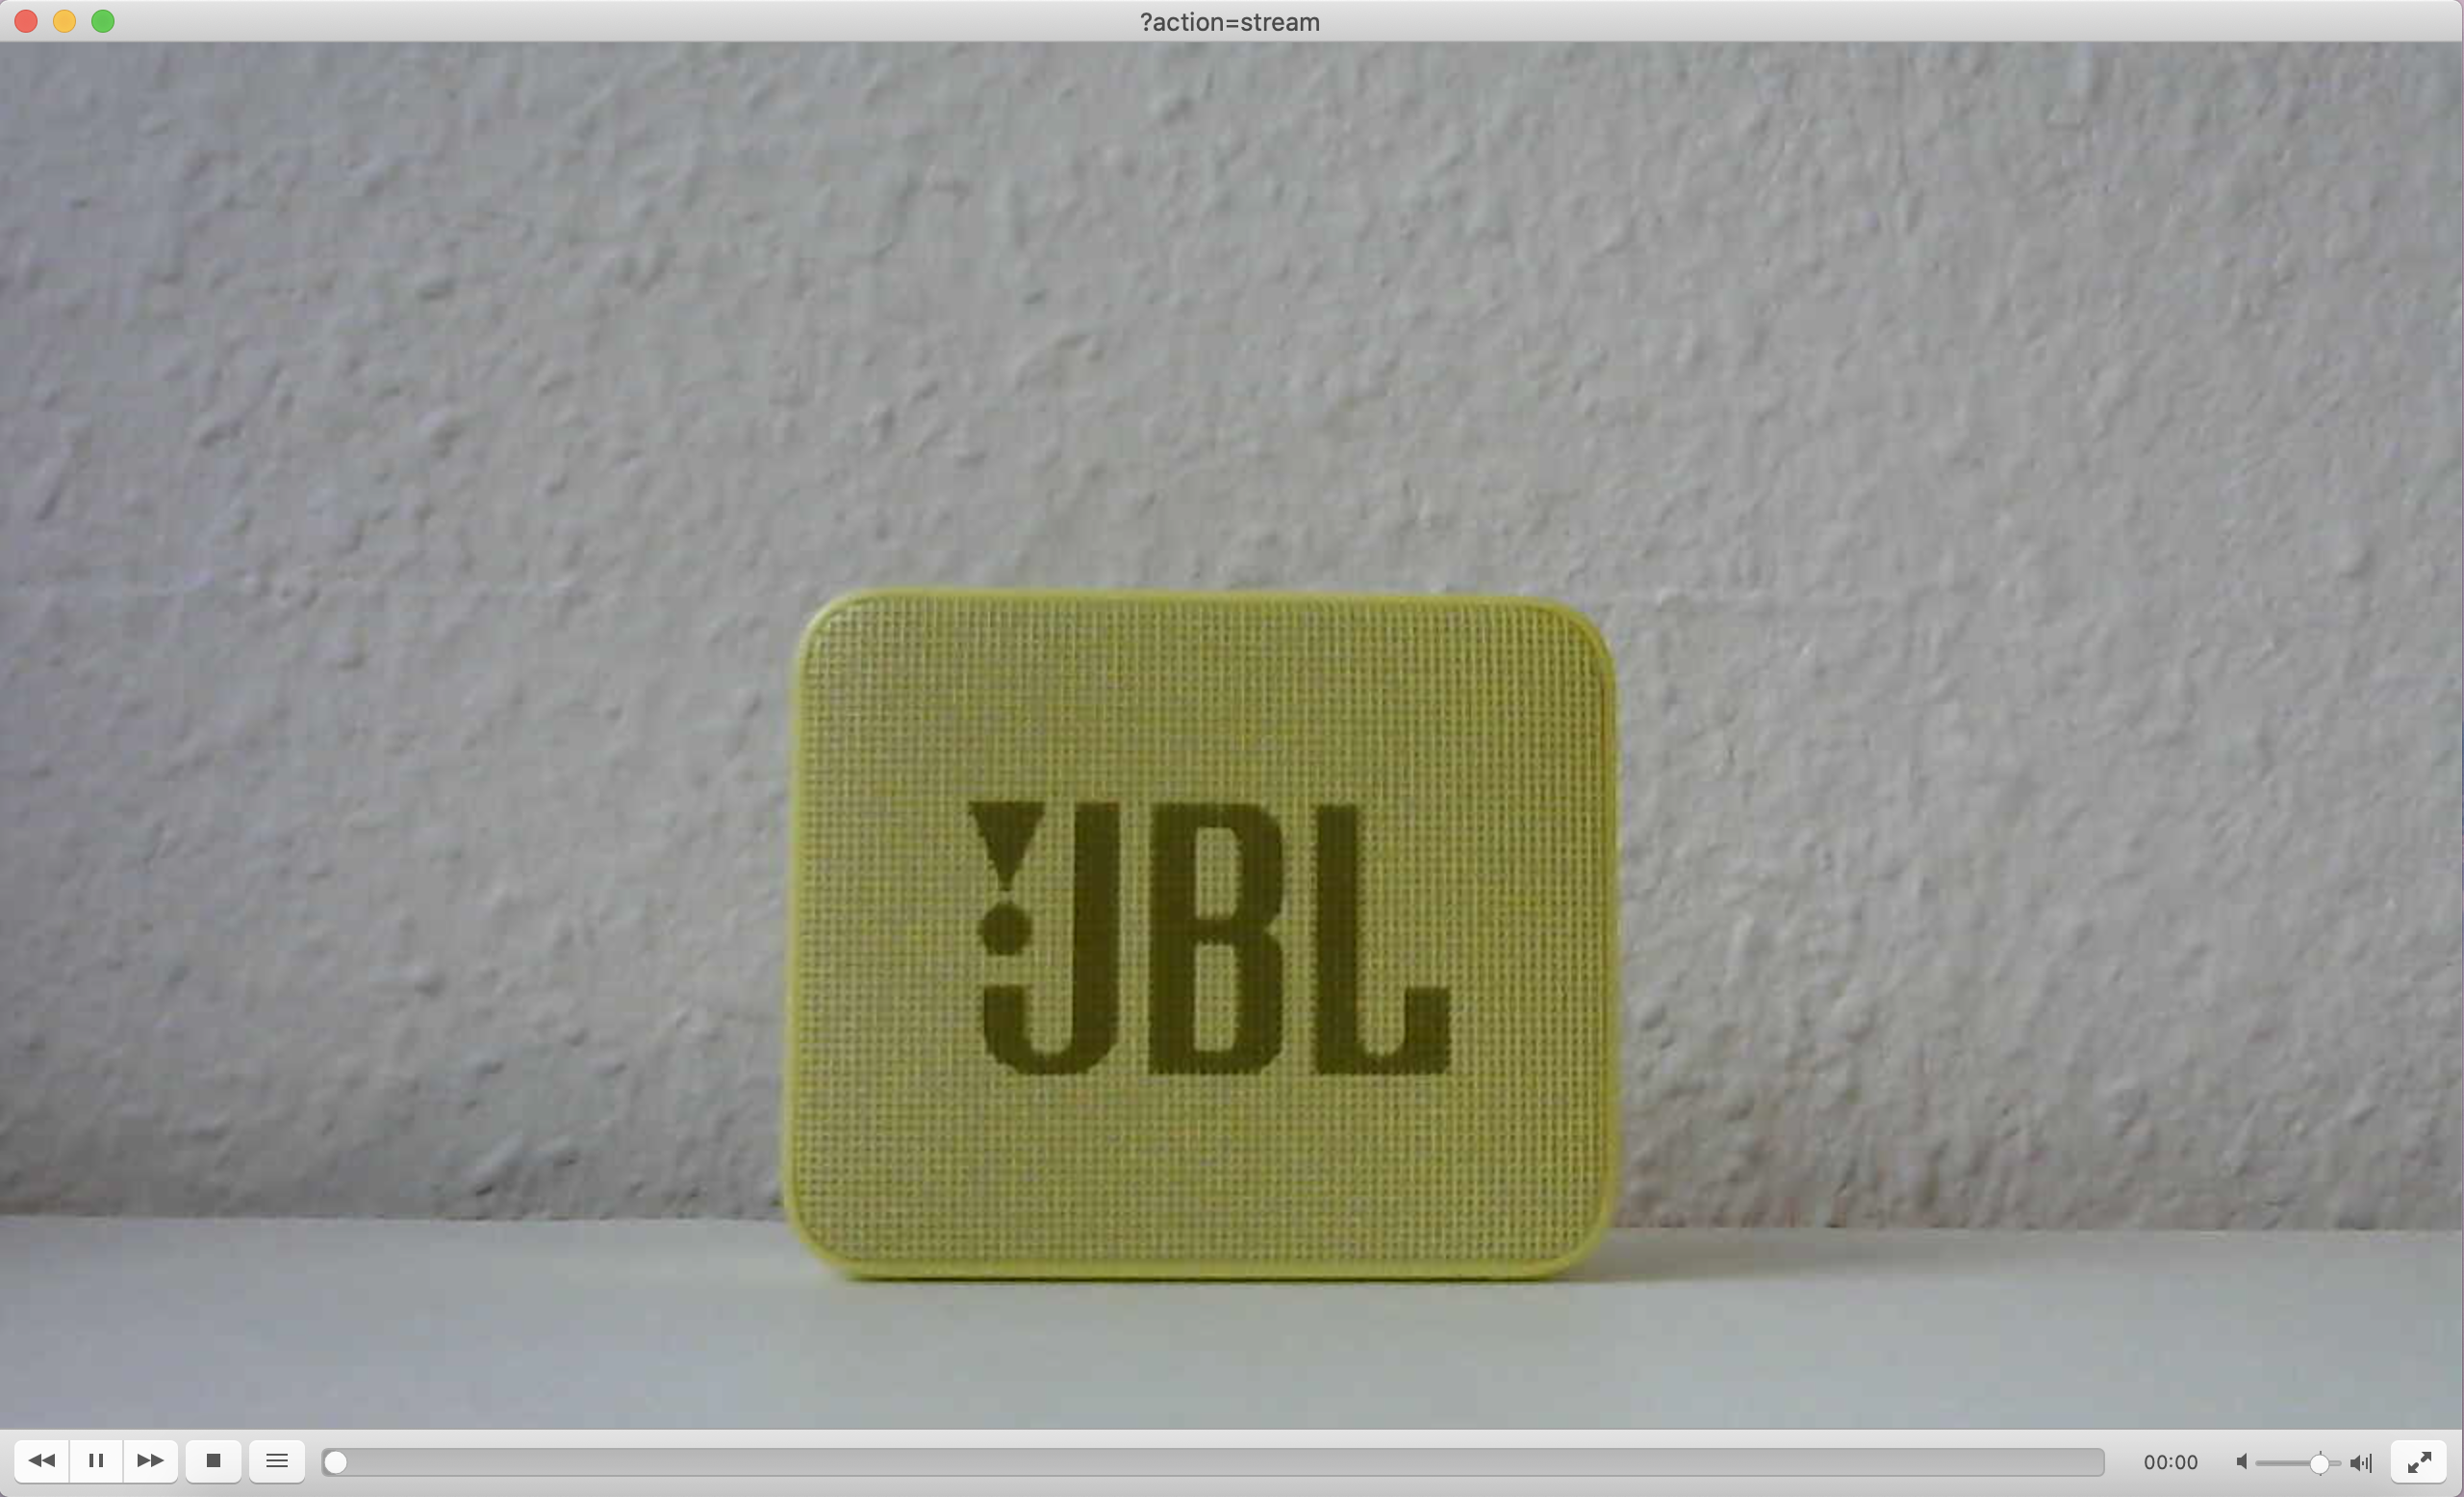
\includegraphics[width=.9\textwidth, trim=4 4 4 4,clip]{images/MJPG-Streamer.png}
	\caption{MJPG-Streamer}
	\label{fig:mjpg}
\end{figure}

At first, we were able to stream video using GStreamer. Subsequently, we couldn’t view the streaming video even though everything is fine from the server-side. We checked the video port from the plug-in configuration file, and we assigned a different port. Still, we couldn’t view the video stream. Fig. \ref{fig:gs} shows the continuous buffering effect. 

\begin{figure}[H]
	\centering
	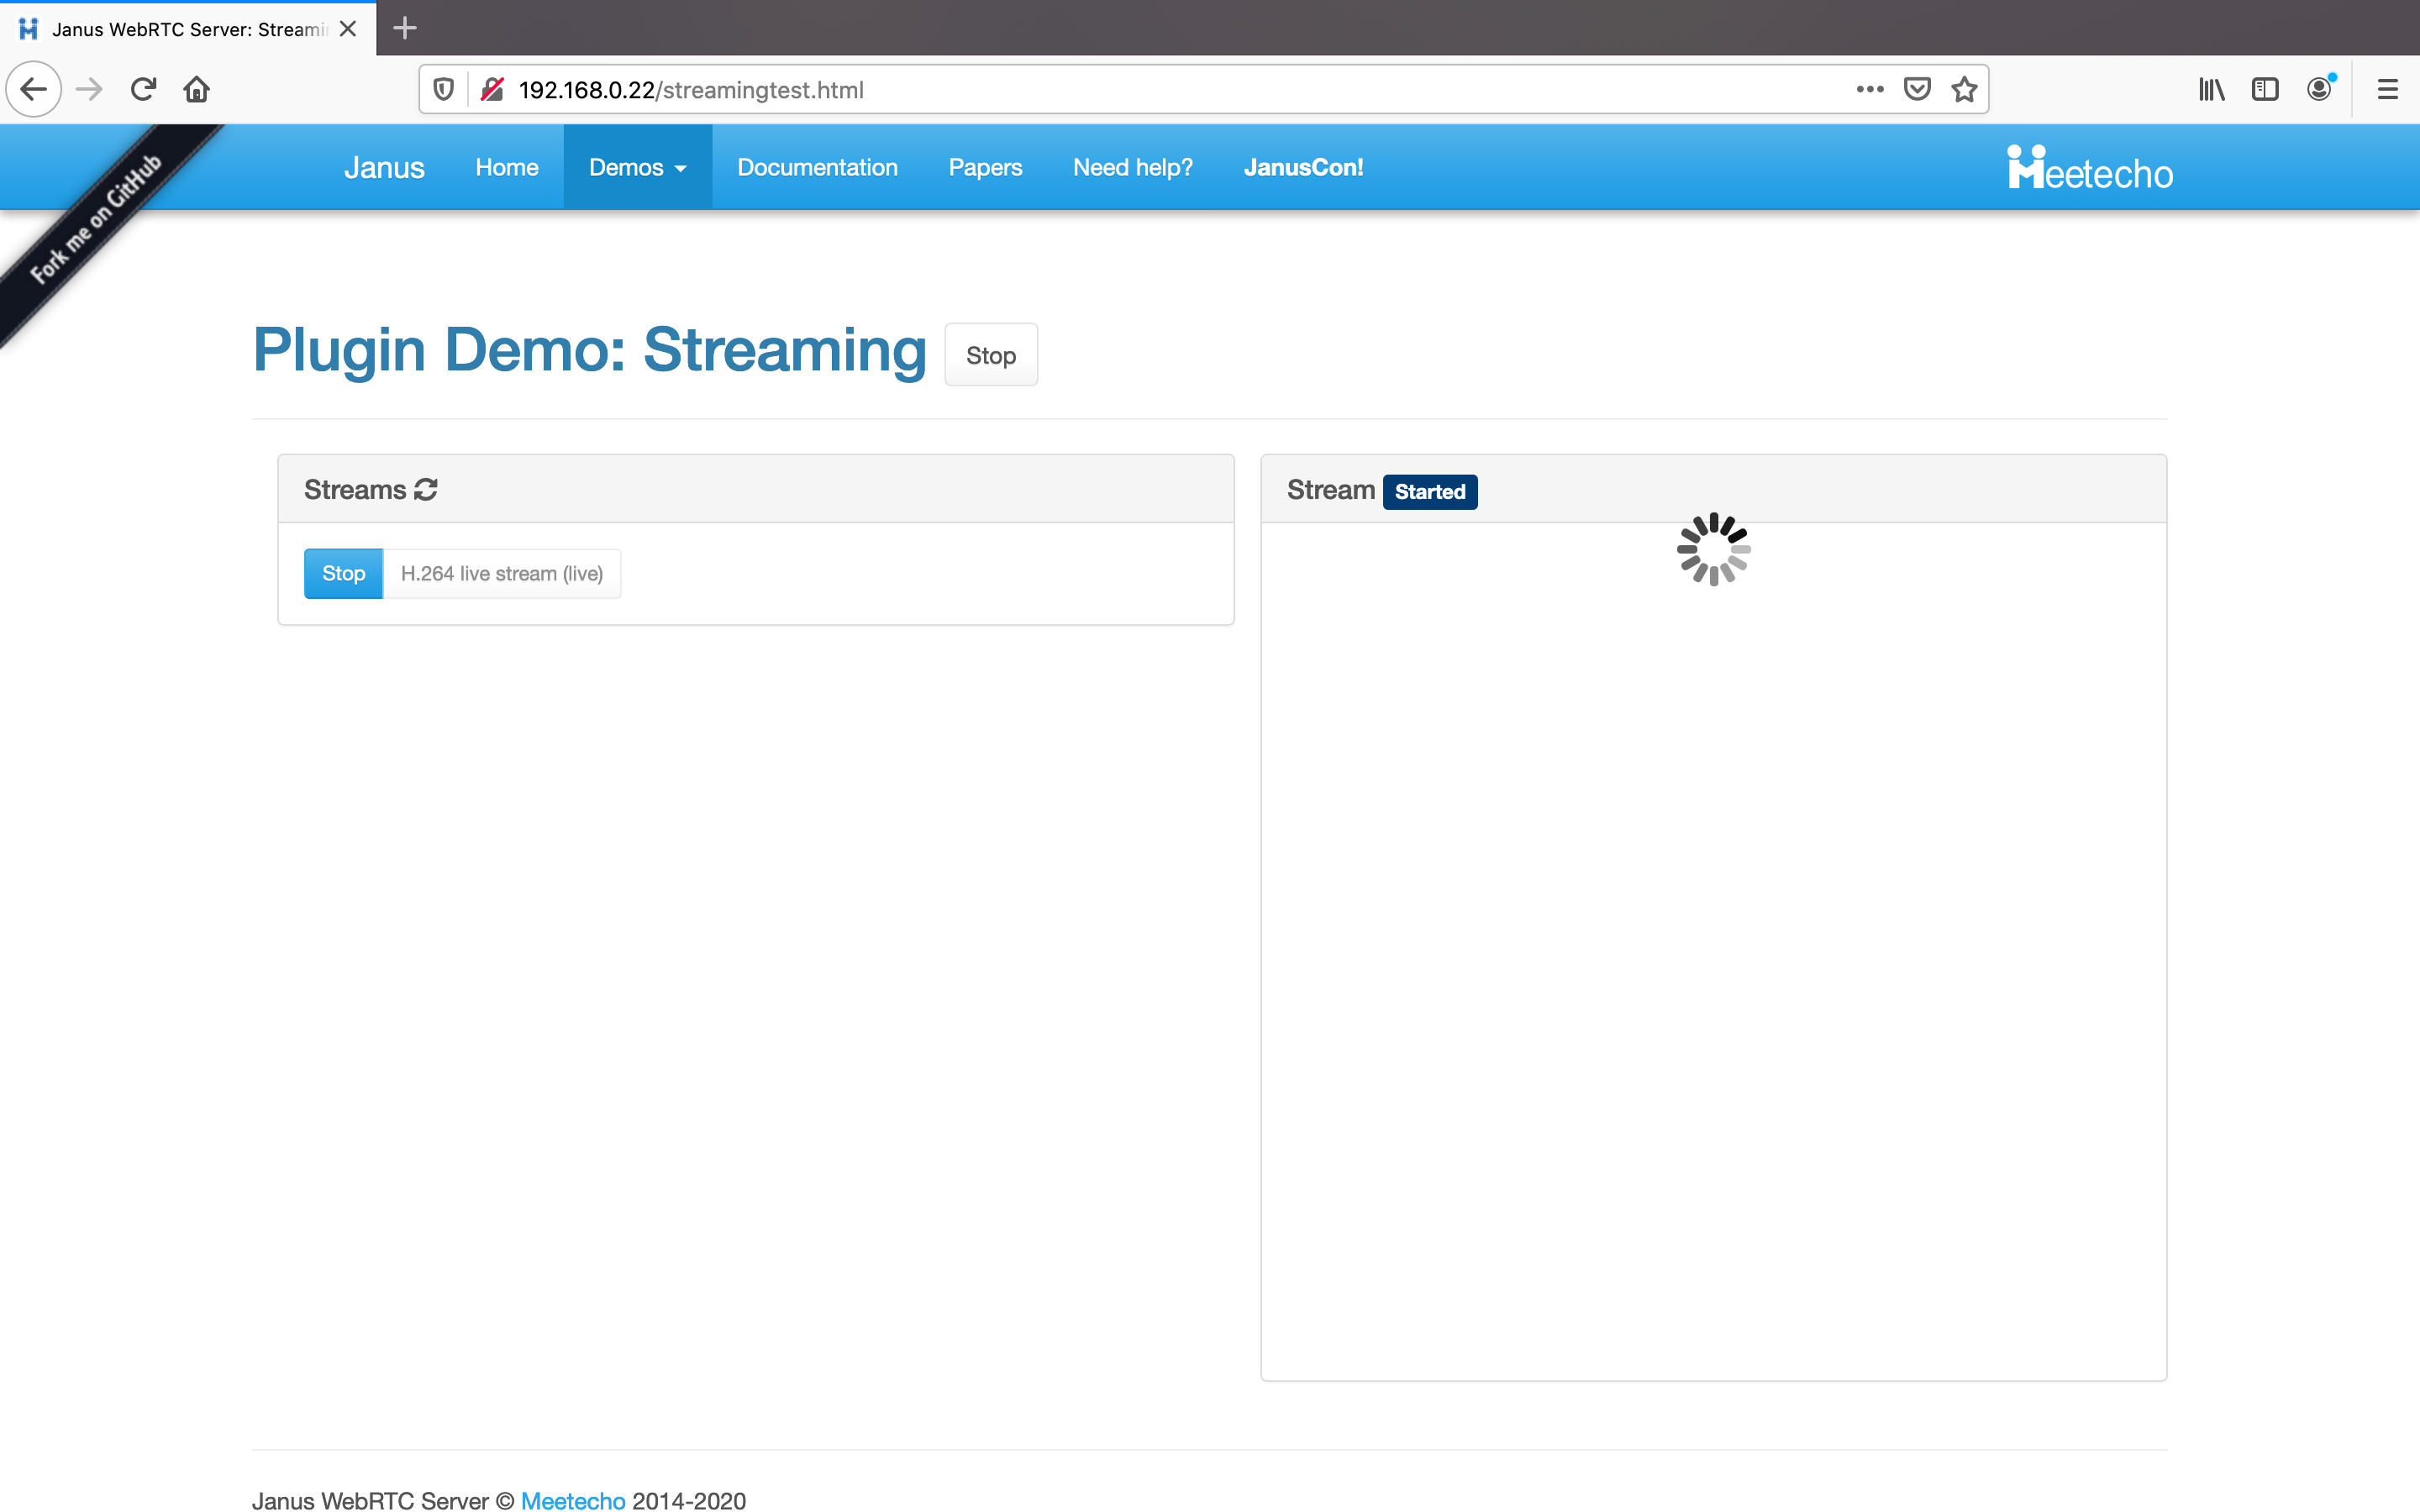
\includegraphics[width=.9\textwidth, trim=4 4 4 4,clip]{images/GStreamer.png}
	\caption{GStreamer H.264}
	\label{fig:gs}
\end{figure}

\subsection{Utilization Comparison of Working Video Streams}

As our main goal in the project is to make a comparison between the multimedia frameworks on RPi3 and RPi4 based on the video quality and resource utilization, we collect the statistics of the multimedia frameworks with its codecs from both RPi3 and RPi4. Based on the statistics, to provide an easy, clear, and descriptive understanding of the data that has been generated, we make use of one of the graphical representations, Boxplot, to provide an illustration of values distributed based on mean, median, and maximum data more precisely in less space. Using Jupyter Notebook we write the Python scripts to draw the boxplots. \par

Here, we make a utilization comparison of RPi3 and RPi4 based on CPU usage, memory usage, and network throughput. \par

For all the multimedia frameworks and codecs, we took seven trials with a time interval of one minute. \par

\textbf{CPU Utilization}:

RPi is a quad-core processor. And when we scrape the metrics for CPU usage of running containers, we get values for all four cores. We calculated the mean for values of four cores to plot the boxplot.

\begin{figure}[H]
	\centering
	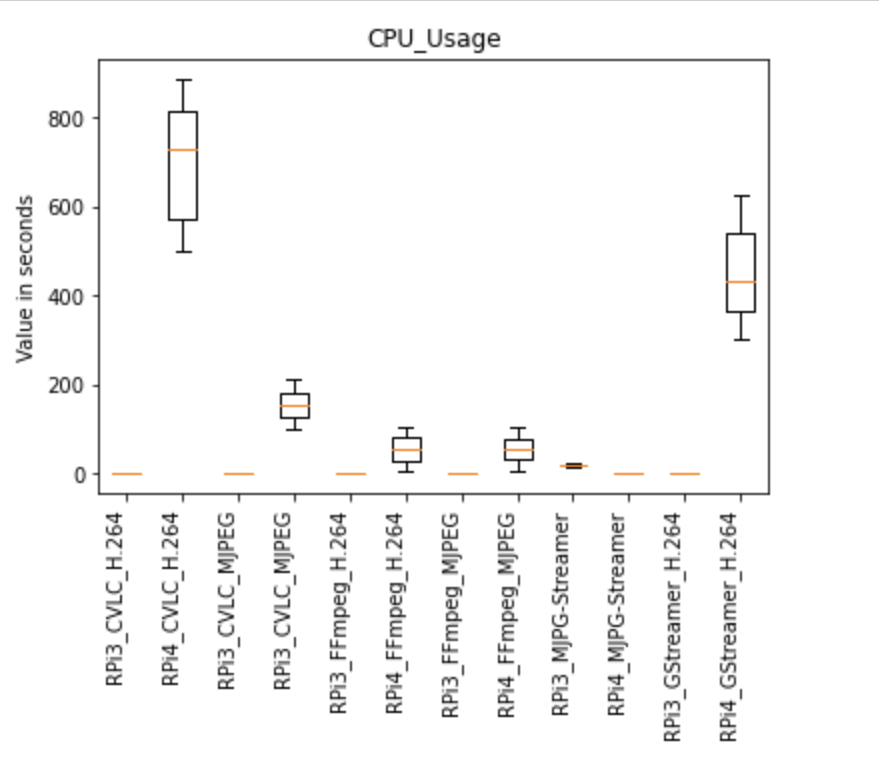
\includegraphics[width=.8\textwidth, trim=4 4 4 4,clip]{images/Boxplots/CPU_Usage.png}
	\caption{CPU Utilization}
	\label{fig:cpu_usage}
\end{figure}

Fig. \ref{fig:cpu_usage} shows the total CPU usage in seconds of all multimedia frameworks with its respective codecs. Unfortunately, in our project, we are unable to view the video stream from the RPi3 except for MJPG-Streamer, which affects the metrics showing no much variation. Hence, we cannot conclude which multimedia framework is best in RPi3. In RPi4, the CPU utilization is high for CVLC (with H.264), which affects the latency, followed by GStreamer (with H.264) because of the running WebRTC container. MJPG-Streamer consumes a minimum amount of CPU followed by FFmpeg (with H.264 and MJPEG), which results in better performance of the system.
  
\textbf{Memory Utilization}:

\begin{figure}[H]
   \centering
   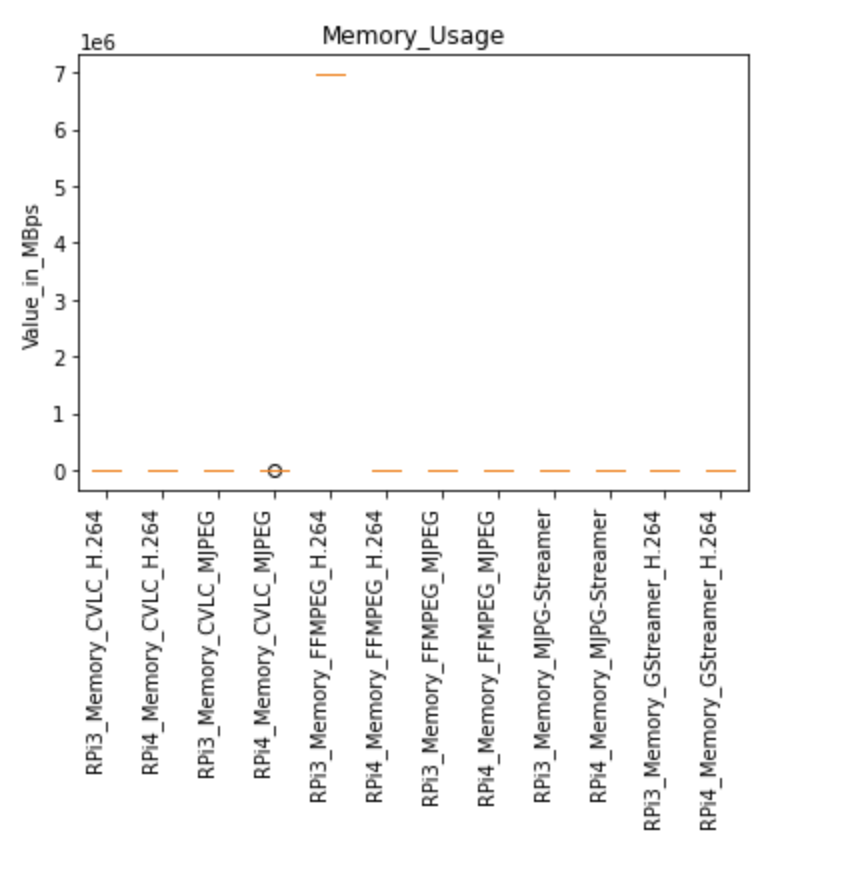
\includegraphics[width=.8\textwidth]{images/Boxplots/Memory_Usage.png}
   \caption{Memory Utilization}
   \label{fig:memory_usage}
\end{figure}

Fig. \ref{fig:memory_usage} shows the total memory usage in Megabytes per second (MBps) of all multimedia frameworks with its respective codecs. Unfortunately, in our project, we are unable to view the video stream from the RPi3 except for MJPG-Streamer, which affects the metrics showing no much variation. Even though there is no video streamed, there is a sudden spike in memory usage for FFmpeg (with H.264), which is uncertain. In RPi4, although all multimedia frameworks have unlimited memory allocation by cAdvisor, they consume a very minimal amount of memory, which is almost fixed across all the frameworks. Hence, we cannot conclude which multimedia framework is best in RPi3 and RPi4 as almost all frameworks consume a minimal amount of memory.

\newpage
\textbf{Network Transmit Total}:

\begin{figure}[H]
   \centering
   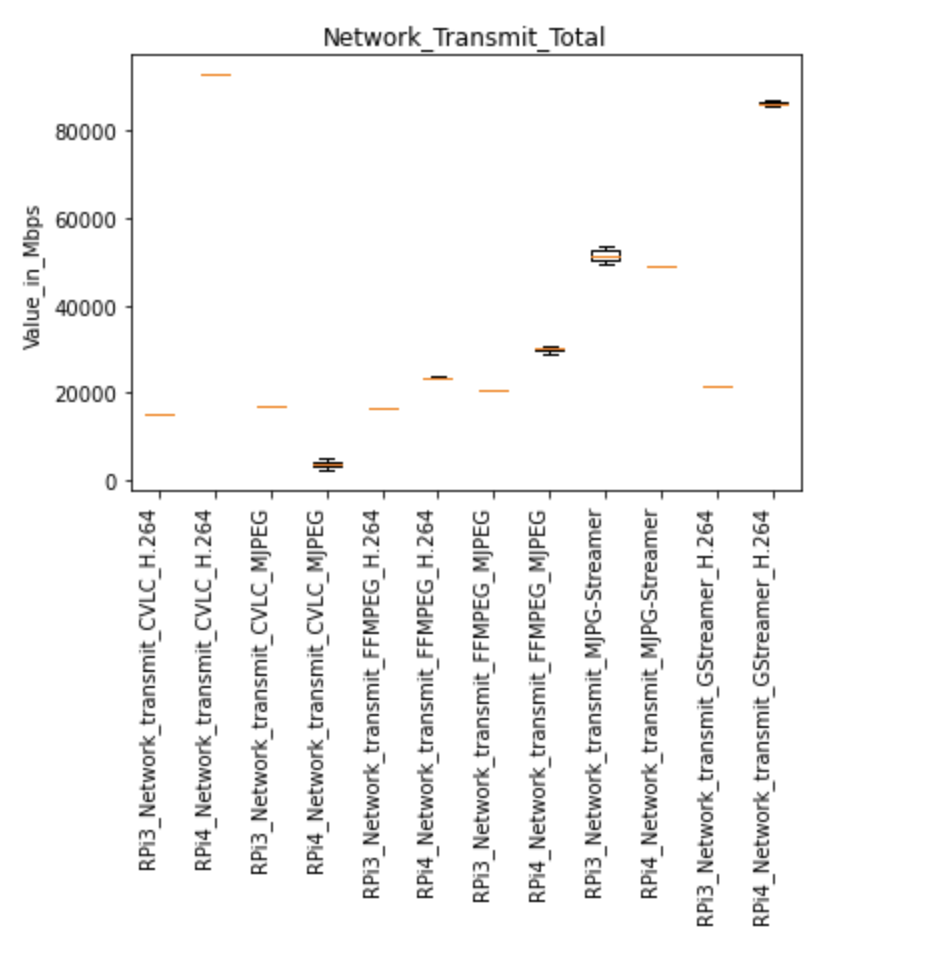
\includegraphics[width=.8\textwidth]{images/Boxplots/Network_Transmit_Total.png}
   \caption{Network Transmit Total}
   \label{fig:network_transmit_total}
\end{figure}

Fig. \ref{fig:network_transmit_total} shows the total network transmission in Megabits per second (Mbps) for all multimedia frameworks with its respective codecs. The higher the bitrate and Network transmission (upstream), the better the video quality, which allows us to send all the allotted video frames over the network. Although we are unable to view the video stream from the RPi3 except for MJPG-Streamer, it shows the variation in values. And from the boxplot, MJPG-Streamer has a higher upstream followed by FFmpeg (with MJPEG), which shows better video quality. In RPi4, GStreamer (with H.264) has a higher upstream because of the running WebRTC container followed by MJPG-Streamer, which shows better video quality.

\newpage
\textbf{Network Receive Total}:

\begin{figure}[H]
   \centering
   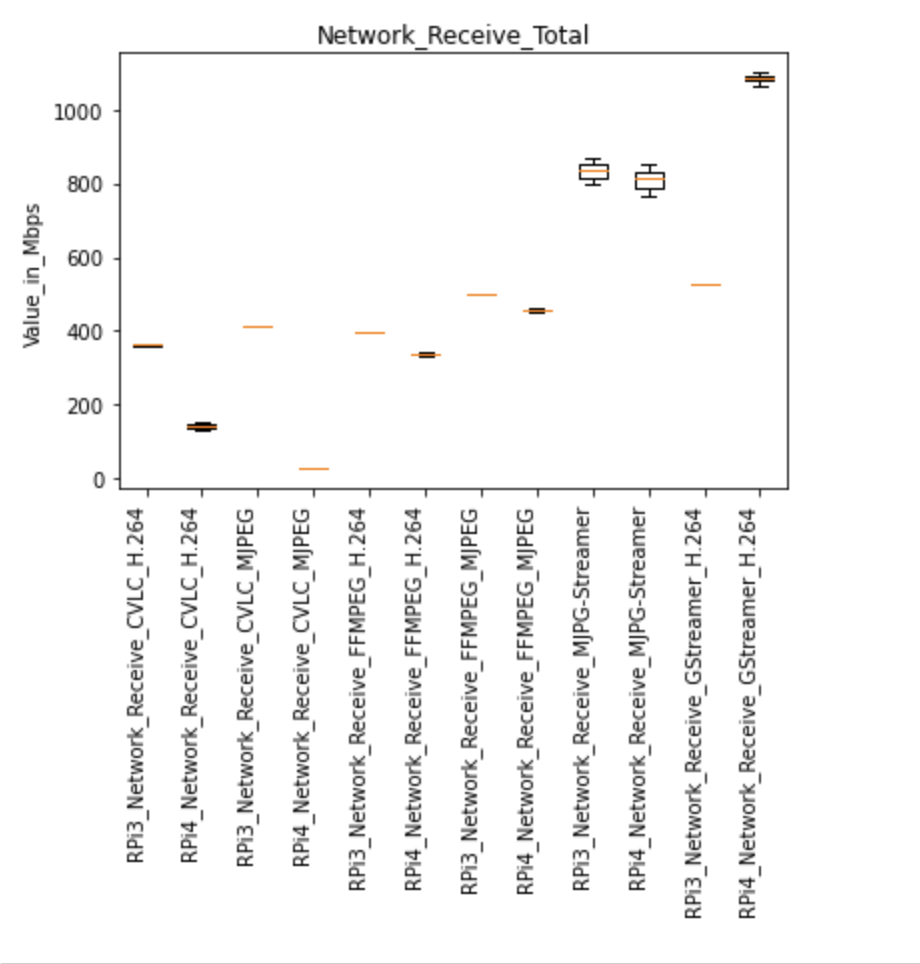
\includegraphics[width=.8\textwidth, trim=4 4 4 4,clip]{images/Boxplots/Network_Receive_Total.png}
   \caption{Network Receive Total}
   \label{fig:network_receive_total}
\end{figure}

Fig. \ref{fig:network_receive_total} shows the total network received in Megabits per second (Mbps) for all multimedia frameworks with its respective codecs. The receiving device receives all the packets sent from the streaming server (RPi).
Although we are unable to view the video stream from the RPi3 except for MJPG-Streamer, it shows the variation in values. And from the boxplot, MJPG-Streamer has higher packets received followed by GStreamer (with H.264), which shows better video quality. In RPi4, GStreamer (with H.264) has higher packets received because of running WebRTC container followed by MJPG-Streamer, which shows better video quality. RPi4 provides better quality of video streaming as its ethernet interface is 100GB, whereas for RPi3 it is 100MB.

The individual boxplots for all the multimedia frameworks and codecs are shown in the Sec. \ref{sec:appendix}.
\section{Conclusion and Future Work}

With the rapid development in the field of Internet and technology, IoT is changing our lives by making things smarter and easier than ever before. This technological improvement has made a positive approach in many fields that are based on a peer-to-peer structure by running on cheap and easily available hardware devices. We built a multimedia system that uses RTP on the RPi4. Our system receives the video stream from the attached camera node, which is encoded and decoded by using two video codecs (H.264 and MJPEG) in four frameworks (CVLC, FFmpeg, MJPG-Streamer, GStreamer) and sent over the network using an RTP. To view the video streamed from RPi, we use the web browser or media-player (VLC) on the receiving device. As our system is virtualized using Docker containers, it makes deployment easy on RPi. \par

By comparing all the frameworks with its respective codecs on RPi3 and RPi4 in terms of resource utilization (CPU, memory, network throughput) and video quality, we arrive at a conclusion that MJPG-Streamer delivers the best performance overall and it only supports the MJPEG codec as WebRTC requires H.264 in RPi4. Followed by is the GStreamer providing the best results in RPi4. And about RPi3, unfortunately in our project, we are unable to view the video stream from the RPi3 except for MJPG-Streamer, which affects the result. This leads to an uncertain situation to determine which multimedia framework is the best on RPi3 and difficult to conclude which RPi is the best. In our project, we realized Janus (WebRTC server) supports very few video codecs and multimedia frameworks, this is why we haven't used MJPEG codec with GStreamer. \par 

Also, we realized, ARM quad-core processor (RPi) does not fully support multimedia frameworks because of no built-in libraries and Graphics Processing Unit (GPU) chip. \par

While our prototype demonstrates the possibilities with current technology using cheap SBCs, future work may provide a more stable foundation in using various other multimedia frameworks for better video streaming quality and added new features.
\clearpage
\appendix
%\section*{Appendix}
\label{sec:appendix}

\subsection*{Steps to start the Multimedia Frameworks and Codecs}

\subsubsection*{CVLC}
To start CVLC, follow the steps shown in Code Listing. \ref{cvlc}

\begin{lstlisting}[caption={Build and run CVLC}, frame=lines, label={cvlc}]
Navigate to the following directory:
/framework-test/ForRaspberryPi/cvlc

$docker build -t cvlc .

$docker run \
  -it \
  --privileged \
  --net=host -v /dev/video0:/dev/video0 \
  -e Ip=<IP of the Receiving Device> cvlc

h264:
$cvlc \
  -vvv v4l2:///dev/video0 \
  --sout "#transcode{vcodec=h264,
  width=640,
  fps=24,
  tune=zerolatency,
  preset=ultrafast}:udp{dst=<IP of the Receiving Device>:2000}" \
  --no-sout-audio

mjpeg:
$cvlc \
  -vvv v4l2:///dev/video0 \
  --sout "#transcode{vcodec=mjpg,
  fps=24}:udp{dst=<IP of the Receiving Device>:2000}" \
  --no-sout-audio

To view the video stream in VLC:
File->Open Network->Enter udp://@:2000
\end{lstlisting}

\subsubsection*{FFmpeg}
To start FFmpeg, follow the steps shown in Code Listing. \ref{ffmpeg}

\begin{lstlisting}[caption={Build and run Ffmpeg}, frame=lines, label={ffmpeg}]
Navigate to the following directory:
/framework-test/ForRaspberryPi/ffmpeg

$docker build -t ffmpeg .

$docker run \
  -it \
  --privileged \
  --net=host -v /dev/video0:/dev/video0 \
  -e Ip=<IP of the Receiving Device> ffmpeg
  
h264:
$ffmpeg \
  -fflags nobuffer \
  -f v4l2 \
  -framerate 30 \
  -i /dev/video0 \
  -vcodec libx264 \
  -preset ultrafast \
  -tune zerolatency \
  -pix_fmt yuv420p \
  -f mpegts udp://<IP of the Receiving Device>:2000?pkt_size=1316

mjpeg:
$ffmpeg \
  -fflags nobuffer \
  -f v4l2 \
  -framerate 30 \
  -i /dev/video0 \
  -vcodec mjpeg \
  -f mjpeg udp://<IP of the Receiving Device>:2000?pkt_size=1316

To view the video stream in VLC:
File->Open Network->Enter udp://@:2000
\end{lstlisting}

\subsubsection*{MJPG-Streamer}
To start MJPG-Streamer, follow the steps shown in Code Listing. \ref{mjpgstreamer}

\begin{lstlisting}[caption={Build and run MJPG-Streamer}, frame=lines, label={mjpgstreamer}]
Navigate to the following directory:
/framework-test/ForRaspberryPi/mjpgstreamer

docker build -t mjpgstreamer .

$docker run \
  -it \
  --privileged \
  --net=host \
  -v /dev/video0:/dev/video0 \
  -e Ip=<IP of the Receiving Device> mjpgstreamer

To view the video stream:
In browser: <IP of the Rpi>:8085
In vlc player: File->Open Network->Enter http://<IP of the Rpi>:8085/?action=stream
\end{lstlisting}

\subsubsection*{GStreamer}
To start GStreamer, follow the steps shown in Code Listing. \ref{gstreamer}

\begin{lstlisting}[caption={Build and run GStreamer}, frame=lines, label={gstreamer}]
To start Janus Server, navigate to the following directory:
/framework-test/ForReceivingDevice/janus_docker_for_testing

$docker run \
  --name=janus \
  --net=host \
  janus 
  
To start GStreamer, navigate to the following directory:
/framework-test/ForRaspberryPi/gstreamer

$docker build -t gstreamer .

$docker run \
  -it \
  --privileged \
  --net=host \
  -v /dev/video0:/dev/video0 \
  -e Ip=<IP of the Receiving Device> gstreamer

h264:
./gstreamer_h264.sh 

To view the video stream:
In browser: <Ip of the Rpi>
Demos->Streaming->Streams list->H.264 live stream(live)->Watch or Listen

To stop the video stream:
Stop
\end{lstlisting}

%Boxplots%
\subsection*{Boxplots showing the Utilization comparison of RPi3 and RPi4}
%CPU%
%\subsubsection{CPU}
\begin{figure}[H]
\centering
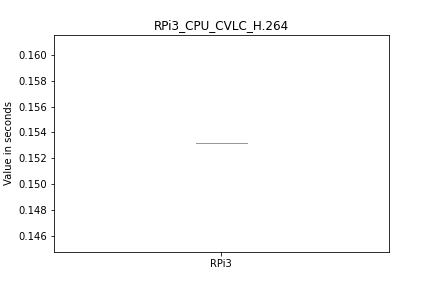
\includegraphics[width=.3\textwidth]{images/Boxplots/RPi3_CPU_CVLC_H_264.png}\hfill
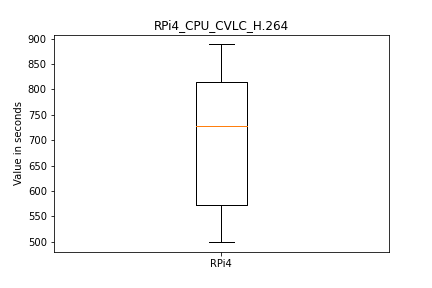
\includegraphics[width=.3\textwidth]{images/Boxplots/RPi4_CPU_CVLC_H_264.png}\hfill
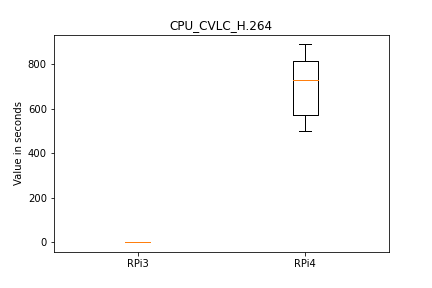
\includegraphics[width=.3\textwidth]{images/Boxplots/CPU_CVLC_H_264.png}
\caption{CPU CVLC H.264}
\label{fig:bp1}
\end{figure}

\begin{figure}[H]
\centering
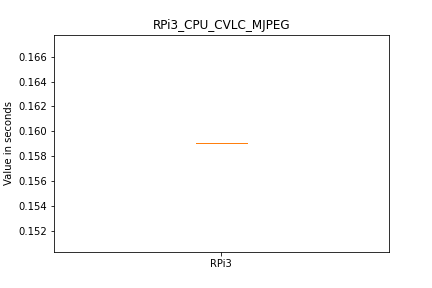
\includegraphics[width=.3\textwidth]{images/Boxplots/RPi3_CPU_CVLC_MJPEG.png}\hfill
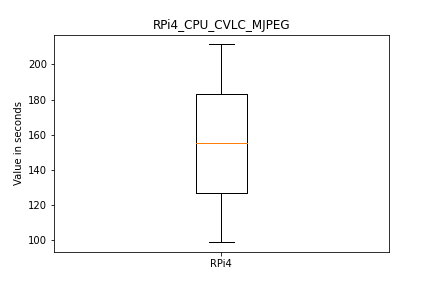
\includegraphics[width=.3\textwidth]{images/Boxplots/RPi4_CPU_CVLC_MJPEG.png}\hfill
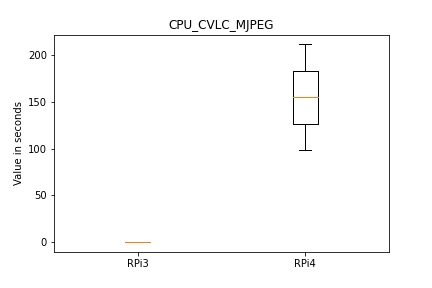
\includegraphics[width=.3\textwidth]{images/Boxplots/CPU_CVLC_MJPEG.png}
\caption{CPU CVLC MJPEG}
\label{fig:bp2}
\end{figure}

\begin{figure}[H]
\centering
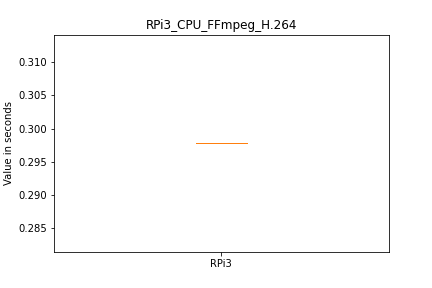
\includegraphics[width=.3\textwidth]{images/Boxplots/RPi3_CPU_FFmpeg_H_264.png}\hfill
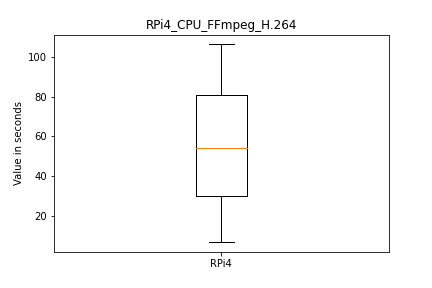
\includegraphics[width=.3\textwidth]{images/Boxplots/RPi4_CPU_FFmpeg_H_264.png}\hfill
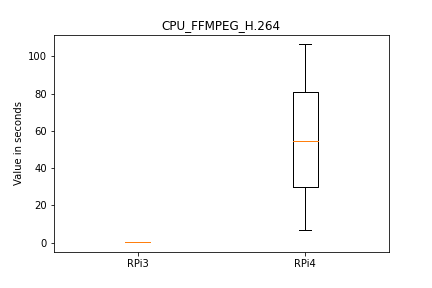
\includegraphics[width=.3\textwidth]{images/Boxplots/CPU_FFmpeg_H_264.png}
\caption{CPU FFmpeg H.264}
\label{fig:bp3}
\end{figure}
\clearpage

\begin{figure}[H]
\centering
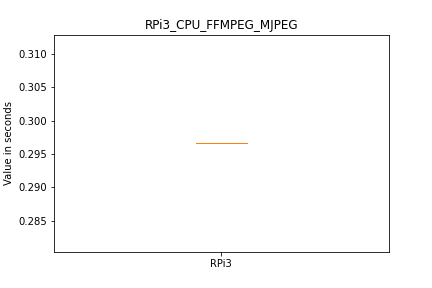
\includegraphics[width=.3\textwidth]{images/Boxplots/RPi3_CPU_FFmpeg_MJPEG.png}\hfill
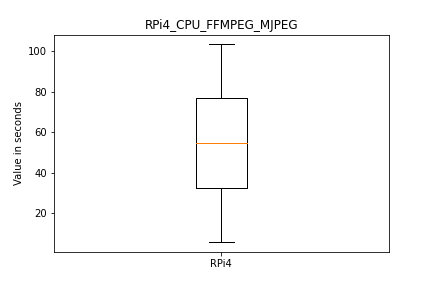
\includegraphics[width=.3\textwidth]{images/Boxplots/RPi4_CPU_FFmpeg_MJPEG.png}\hfill
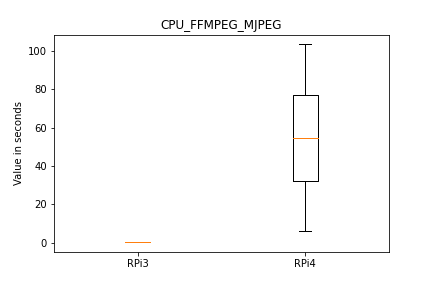
\includegraphics[width=.3\textwidth]{images/Boxplots/CPU_FFmpeg_MJPEG.png}
\caption{CPU FFmpeg MJPEG}
\label{fig:bp4}
\end{figure}

\begin{figure}[H]
\centering
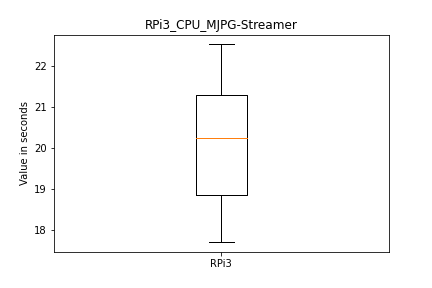
\includegraphics[width=.3\textwidth]{images/Boxplots/RPi3_CPU_MJPG-Streamer.png}\hfill
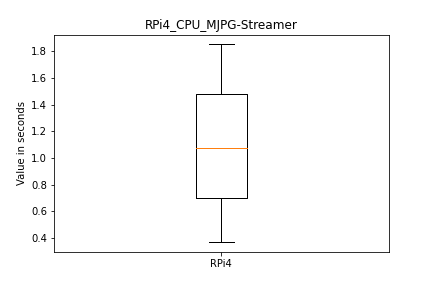
\includegraphics[width=.3\textwidth]{images/Boxplots/RPi4_CPU_MJPG-Streamer.png}\hfill
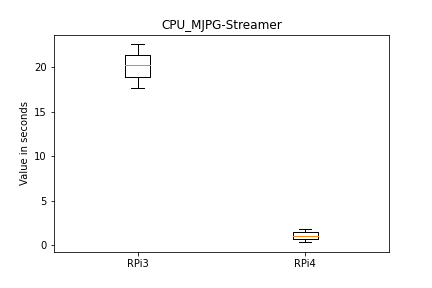
\includegraphics[width=.3\textwidth]{images/Boxplots/CPU_MJPG-Streamer.png}
\caption{CPU MJPG-Streamer}
\label{fig:bp5}
\end{figure}

\begin{figure}[H]
\centering
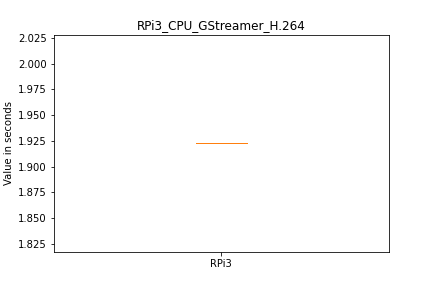
\includegraphics[width=.3\textwidth]{images/Boxplots/RPi3_CPU_GStreamer_H_264.png}\hfill
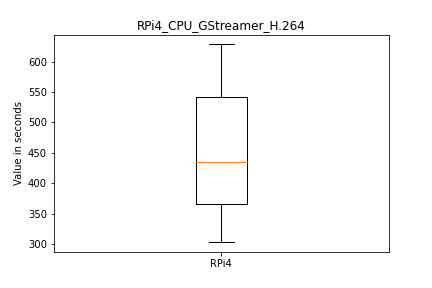
\includegraphics[width=.3\textwidth]{images/Boxplots/RPi4_CPU_GStreamer_H_264.png}\hfill
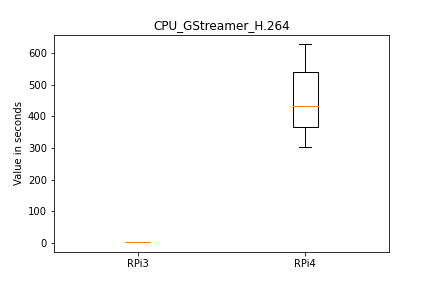
\includegraphics[width=.3\textwidth]{images/Boxplots/CPU_GStreamer_H_264.png}
\caption{CPU GStreamer H.264}
\label{fig:bp6}
\end{figure}

%Memory%
%\subsubsection{Memory}
\begin{figure}[H]
\centering
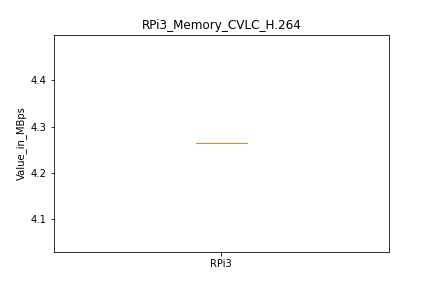
\includegraphics[width=.3\textwidth]{images/Boxplots/RPi3_Memory_CVLC_H_264.png}\hfill
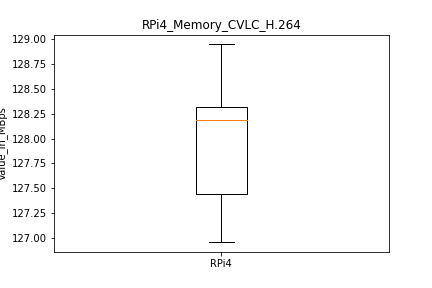
\includegraphics[width=.3\textwidth]{images/Boxplots/RPi4_Memory_CVLC_H_264.png}\hfill
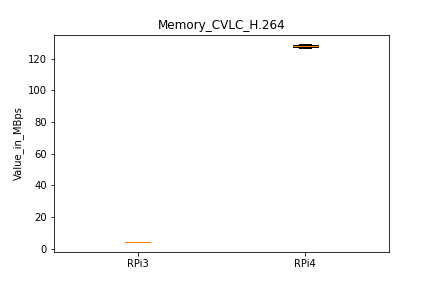
\includegraphics[width=.3\textwidth]{images/Boxplots/Memory_CVLC_H_264.png}
\caption{Memory CVLC H.264}
\label{fig:bp7}
\end{figure}

\begin{figure}[H]
\centering
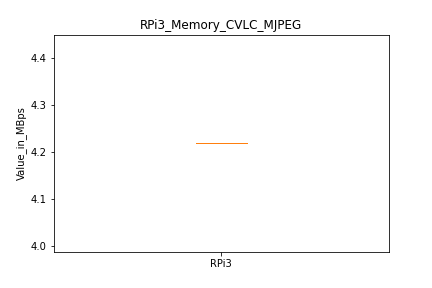
\includegraphics[width=.3\textwidth]{images/Boxplots/RPi3_Memory_CVLC_MJPEG.png}\hfill
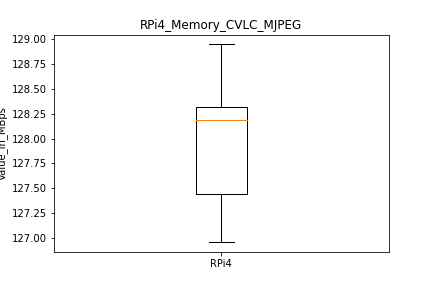
\includegraphics[width=.3\textwidth]{images/Boxplots/RPi4_Memory_CVLC_MJPEG.png}\hfill
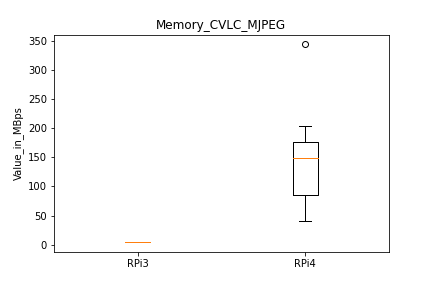
\includegraphics[width=.3\textwidth]{images/Boxplots/Memory_CVLC_MJPEG.png}
\caption{Memory CVLC MJPEG}
\label{fig:bp8}
\end{figure}
\clearpage

\begin{figure}[H]
\centering
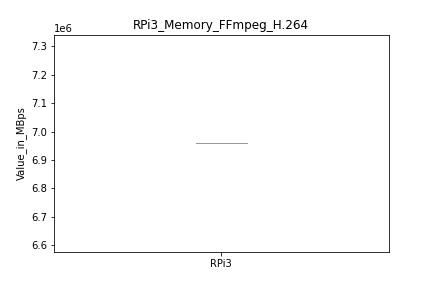
\includegraphics[width=.3\textwidth]{images/Boxplots/RPi3_Memory_FFmpeg_H_264.png}\hfill
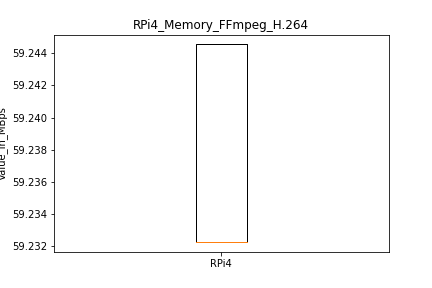
\includegraphics[width=.3\textwidth]{images/Boxplots/RPi4_Memory_FFmpeg_H_264.png}\hfill
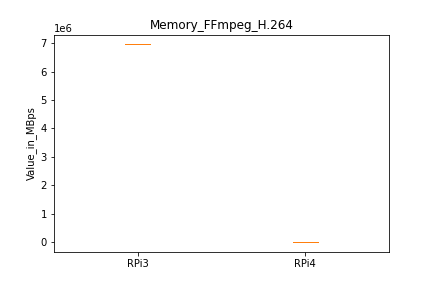
\includegraphics[width=.3\textwidth]{images/Boxplots/Memory_FFmpeg_H_264.png}
\caption{Memory FFmpeg H.264}
\label{fig:bp9}
\end{figure}

\begin{figure}[H]
\centering
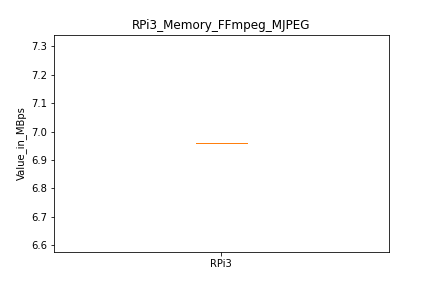
\includegraphics[width=.3\textwidth]{images/Boxplots/RPi3_Memory_FFmpeg_MJPEG.png}\hfill
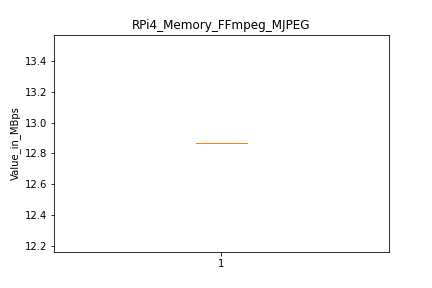
\includegraphics[width=.3\textwidth]{images/Boxplots/RPi4_Memory_FFmpeg_MJPEG.png}\hfill
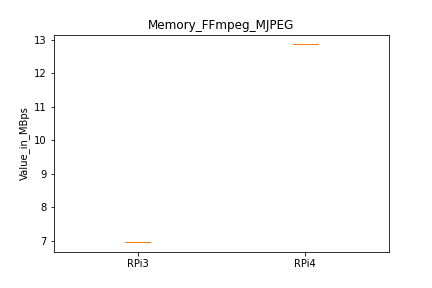
\includegraphics[width=.3\textwidth]{images/Boxplots/Memory_FFmpeg_MJPEG.png}
\caption{Memory FFmpeg MJPEG}
\label{fig:bp10}
\end{figure}

\begin{figure}[H]
\centering
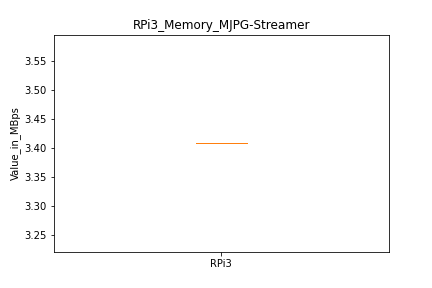
\includegraphics[width=.3\textwidth]{images/Boxplots/RPi3_Memory_MJPG-Streamer.png}\hfill
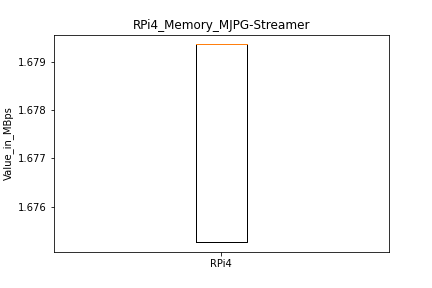
\includegraphics[width=.3\textwidth]{images/Boxplots/RPi4_Memory_MJPG-Streamer.png}\hfill
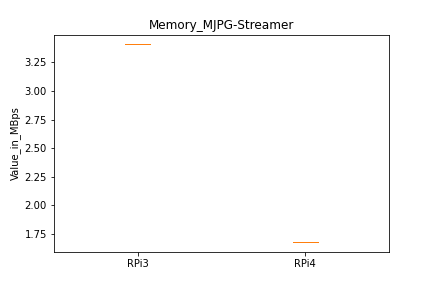
\includegraphics[width=.3\textwidth]{images/Boxplots/Memory_MJPG-Streamer.png}
\caption{Memory MJPG-Streamer}
\label{fig:bp11}
\end{figure}

\begin{figure}[H]
\centering
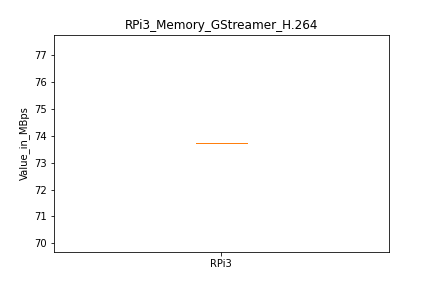
\includegraphics[width=.3\textwidth]{images/Boxplots/RPi3_Memory_GStreamer_H_264.png}\hfill
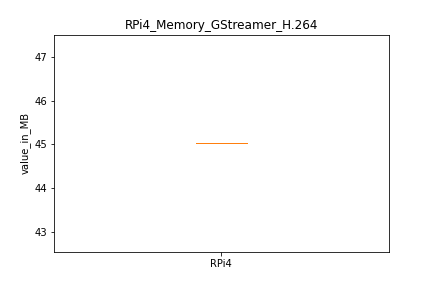
\includegraphics[width=.3\textwidth]{images/Boxplots/RPi4_Memory_GStreamer_H_264.png}\hfill
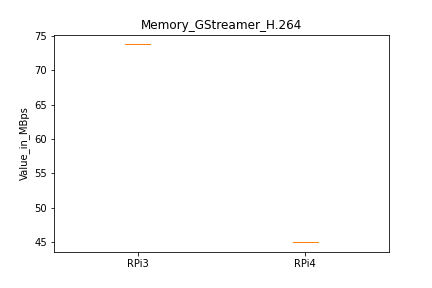
\includegraphics[width=.3\textwidth]{images/Boxplots/Memory_GStreamer_H_264.png}
\caption{Memory GStreamer H.264}
\label{fig:bp12}
\end{figure}

%Network Receive%
%\subsubsection{Network Receiver}
\begin{figure}[H]
\centering
\includegraphics[width=.3\textwidth]{images/Boxplots/RPi3_Network_Receive_CVLC_H_264.png}\hfill
\includegraphics[width=.3\textwidth]{images/Boxplots/RPi4_Network_Receive_CVLC_H_264.png}\hfill
\includegraphics[width=.3\textwidth]{images/Boxplots/Network_Receive_CVLC_H_264.png}
\caption{Network Receive CVLC H.264}
\label{fig:bp13}
\end{figure}
\clearpage

\begin{figure}[H]
\centering
\includegraphics[width=.3\textwidth]{images/Boxplots/RPi3_Network_Receive_CVLC_MJPEG.png}\hfill
\includegraphics[width=.3\textwidth]{images/Boxplots/RPi4_Network_Receive_CVLC_MJPEG.png}\hfill
\includegraphics[width=.3\textwidth]{images/Boxplots/Network_Receive_CVLC_MJPEG.png}
\caption{Network Receive CVLC MJPEG}
\label{fig:bp14}
\end{figure}

\begin{figure}[H]
\centering
\includegraphics[width=.3\textwidth]{images/Boxplots/RPi3_Network_Receive_FFmpeg_H_264.png}\hfill
\includegraphics[width=.3\textwidth]{images/Boxplots/RPi4_Network_Receive_FFmpeg_H_264.png}\hfill
\includegraphics[width=.3\textwidth]{images/Boxplots/Network_Receive_FFmpeg_H_264.png}
\caption{Network Receive FFmpeg H.264}
\label{fig:bp14}
\end{figure}

\begin{figure}[H]
\centering
\includegraphics[width=.3\textwidth]{images/Boxplots/RPi3_Network_Receive_FFmpeg_MJPEG.png}\hfill
\includegraphics[width=.3\textwidth]{images/Boxplots/RPi4_Network_Receive_FFmpeg_MJPEG.png}\hfill
\includegraphics[width=.3\textwidth]{images/Boxplots/Network_Receive_FFmpeg_MJPEG.png}
\caption{Network Receive FFmpeg MJPEG}
\label{fig:bp15}
\end{figure}

\begin{figure}[H]
\centering
\includegraphics[width=.3\textwidth]{images/Boxplots/RPi3_Network_Receive_MJPG-Streamer.png}\hfill
\includegraphics[width=.3\textwidth]{images/Boxplots/RPi4_Network_Receive_MJPG-Streamer.png}\hfill
\includegraphics[width=.3\textwidth]{images/Boxplots/Network_Receive_MJPG-Streamer.png}
\caption{Network Receive MJPG-Streamer}
\label{fig:bp16}
\end{figure}

\begin{figure}[H]
\centering
\includegraphics[width=.3\textwidth]{images/Boxplots/RPi3_Network_Receive_GStreamer.png}\hfill
\includegraphics[width=.3\textwidth]{images/Boxplots/RPi4_Network_Receive_GStreamer.png}\hfill
\includegraphics[width=.3\textwidth]{images/Boxplots/Network_Receive_GStreamer_H_264.png}
\caption{Network Receive GStreamer H.264}
\label{fig:bp17}
\end{figure}

%Network Tranmsit%
%\subsubsection{Network Tranmsit}
\begin{figure}[H]
\centering
\includegraphics[width=.3\textwidth]{images/Boxplots/RPi3_Network_Transmit_CVLC_H_264.png}\hfill
\includegraphics[width=.3\textwidth]{images/Boxplots/RPi4_Network_Transmit_CVLC_H_264.png}\hfill
\includegraphics[width=.3\textwidth]{images/Boxplots/Network_Transmit_CVLC_H_264.png}
\caption{Network Transmit CVLC H.264}
\label{fig:bp18}
\end{figure}

\begin{figure}[H]
\centering
\includegraphics[width=.3\textwidth]{images/Boxplots/RPi3_Network_Transmit_CVLC_MJPEG.png}\hfill
\includegraphics[width=.3\textwidth]{images/Boxplots/RPi4_Network_Transmit_CVLC_MJPEG.png}\hfill
\includegraphics[width=.3\textwidth]{images/Boxplots/Network_Transmit_CVLC_MJPEG.png}
\caption{Network Transmit CVLC MJPEG}
\label{fig:bp19}
\end{figure}

\begin{figure}[H]
\centering
\includegraphics[width=.3\textwidth]{images/Boxplots/RPi3_Network_Transmit_FFmpeg_H_264.png}\hfill
\includegraphics[width=.3\textwidth]{images/Boxplots/RPi4_Network_Transmit_FFmpeg_H_264.png}\hfill
\includegraphics[width=.3\textwidth]{images/Boxplots/Network_Transmit_FFmpeg_H_264.png}
\caption{Network Transmit FFmpeg H.264}
\label{fig:bp20}
\end{figure}

\begin{figure}[H]
\centering
\includegraphics[width=.3\textwidth]{images/Boxplots/RPi3_Network_Transmit_FFmpeg_MJPEG.png}\hfill
\includegraphics[width=.3\textwidth]{images/Boxplots/RPi4_Network_Transmit_FFmpeg_MJPEG.png}\hfill
\includegraphics[width=.3\textwidth]{images/Boxplots/Network_Transmit_FFmpeg_MJPEG.png}
\caption{Network Transmit FFmpeg MJPEG}
\label{fig:bp21}
\end{figure}

\begin{figure}[H]
\centering
\includegraphics[width=.3\textwidth]{images/Boxplots/RPi3_Network_Transmit_MJPG-Streamer.png}\hfill
\includegraphics[width=.3\textwidth]{images/Boxplots/RPi4_Network_Transmit_MJPG-Streamer.png}\hfill
\includegraphics[width=.3\textwidth]{images/Boxplots/Network_Transmit_MJPG-Streamer.png}
\caption{Network Transmit MJPG-Streamer}
\label{fig:bp22}
\end{figure}

\begin{figure}[H]
\centering
\includegraphics[width=.3\textwidth]{images/Boxplots/RPi3_Network_Transmit_GStreamer_H_264.png}\hfill
\includegraphics[width=.3\textwidth]{images/Boxplots/RPi4_Network_Transmit_GStreamer_H_264.png}\hfill
\includegraphics[width=.3\textwidth]{images/Boxplots/Network_Transmit_GStreamer_H_264.png}
\caption{Network Transmit GStreamer H.264}
\label{fig:bp23}
\end{figure}

\clearpage
%
%===============================================================================
% LATEX-Dokument: Literaturverzeichnis
%===============================================================================
%
\newpage
\phantomsection
% Einstellungen f\"{u}r Literaturverzeichnis
\addcontentsline{toc}{section}{\bibname}

\bibliographystyle{IEEEtran}
% argument is your BibTeX string definitions and bibliography database(s)
\bibliography{literature/bib}
% Nutzung von Bibtex:
% hier den bib-file einbinden
%
% GATHER{bibfile.bib}
% \footnotesize
% \bibliography{bibfile}
% ansonsten: bbl als tex Datei einbinden
 %\input{KTR-Seminar-Literatur.tex}
%===============================================================================
% LATEX-Dokument: Literaturverzeichnis
%===============================================================================

\newpage
\phantomsection
\addcontentsline{toc}{section}{Personal Reports}

\includepdf[pages=-]{../../personal/\student/report_1.pdf}
\includepdf[pages=-]{../../personal/\student/report_2.pdf}
\includepdf[pages=-]{../../personal/\student/report_3.pdf}

\end{document}
